\section*{Введение}

В данной лабораторной работе рассматриваются методы жёсткой фильтрации сигналов в частотной области. Фильтрация является важным инструментом обработки сигналов, позволяющим выделять полезную информацию из зашумлённых данных.

\textbf{Цель работы:} изучение методов жёсткой фильтрации сигналов с использованием преобразования Фурье и исследование эффективности различных подходов к устранению помех.

\textbf{Задачи:}
\begin{enumerate}
    \item Исследование фильтрации высоких частот
    \item Изучение фильтрации специфических частот
    \item Анализ фильтрации низких частот
    \item Применение методов фильтрации к реальному аудиосигналу
\end{enumerate}

\section*{Задание 1. Жёсткие фильтры}

\subsection*{Постановка задачи}

Рассматривается функция $g(t)$ такая, что:
\begin{equation}
g(t) = \begin{cases}
a, & t \in [t_1, t_2] \\
0, & t \notin [t_1, t_2]
\end{cases}
\end{equation}

где $a, t_1, t_2$ — заданные параметры, причём $t_1 < t_2$.

Зашумлённая версия сигнала задаётся как:
\begin{equation}
u(t) = g(t) + b \cdot (\text{rand}(t) - 0.5) + c \cdot \sin(d \cdot t)
\end{equation}

где:
\begin{itemize}
    \item $b \cdot (\text{rand}(t) - 0.5)$ — случайный шум
    \item $c \cdot \sin(d \cdot t)$ — гармоническая помеха
\end{itemize}

\subsection*{Методология фильтрации}

Для выполнения жёсткой фильтрации используется следующий алгоритм:
\begin{enumerate}
    \item Вычисление Фурье-образа сигнала $u(t)$
    \item Обнуление значений Фурье-образа на выбранных диапазонах частот
    \item Восстановление сигнала с помощью обратного преобразования Фурье
\end{enumerate}

\subsection*{Фильтрация высоких частот}

В данном разделе исследуется фильтрация высоких частот при $c = 0$. 

\textbf{Параметры эксперимента:}
\begin{itemize}
    \item $a = 1.0$ — амплитуда исходного сигнала
    \item $t_1 = -2.0$, $t_2 = 2.0$ — границы прямоугольного импульса
    \item $T = 20.0$ — большой интервал времени
    \item $dt = 0.01$ — маленький шаг дискретизации
    \item $b = 0.3$ — амплитуда случайного шума
\end{itemize}

\textbf{Метод фильтрации:}
\begin{itemize}
    \item Оставляем Фурье-образ неизменным для диапазона частот $[-\nu_0, \nu_0]$
    \item Обнуляем значения на всех остальных частотах
    \item Выполняем обратное преобразование Фурье
\end{itemize}

\begin{figure}[H]
\centering
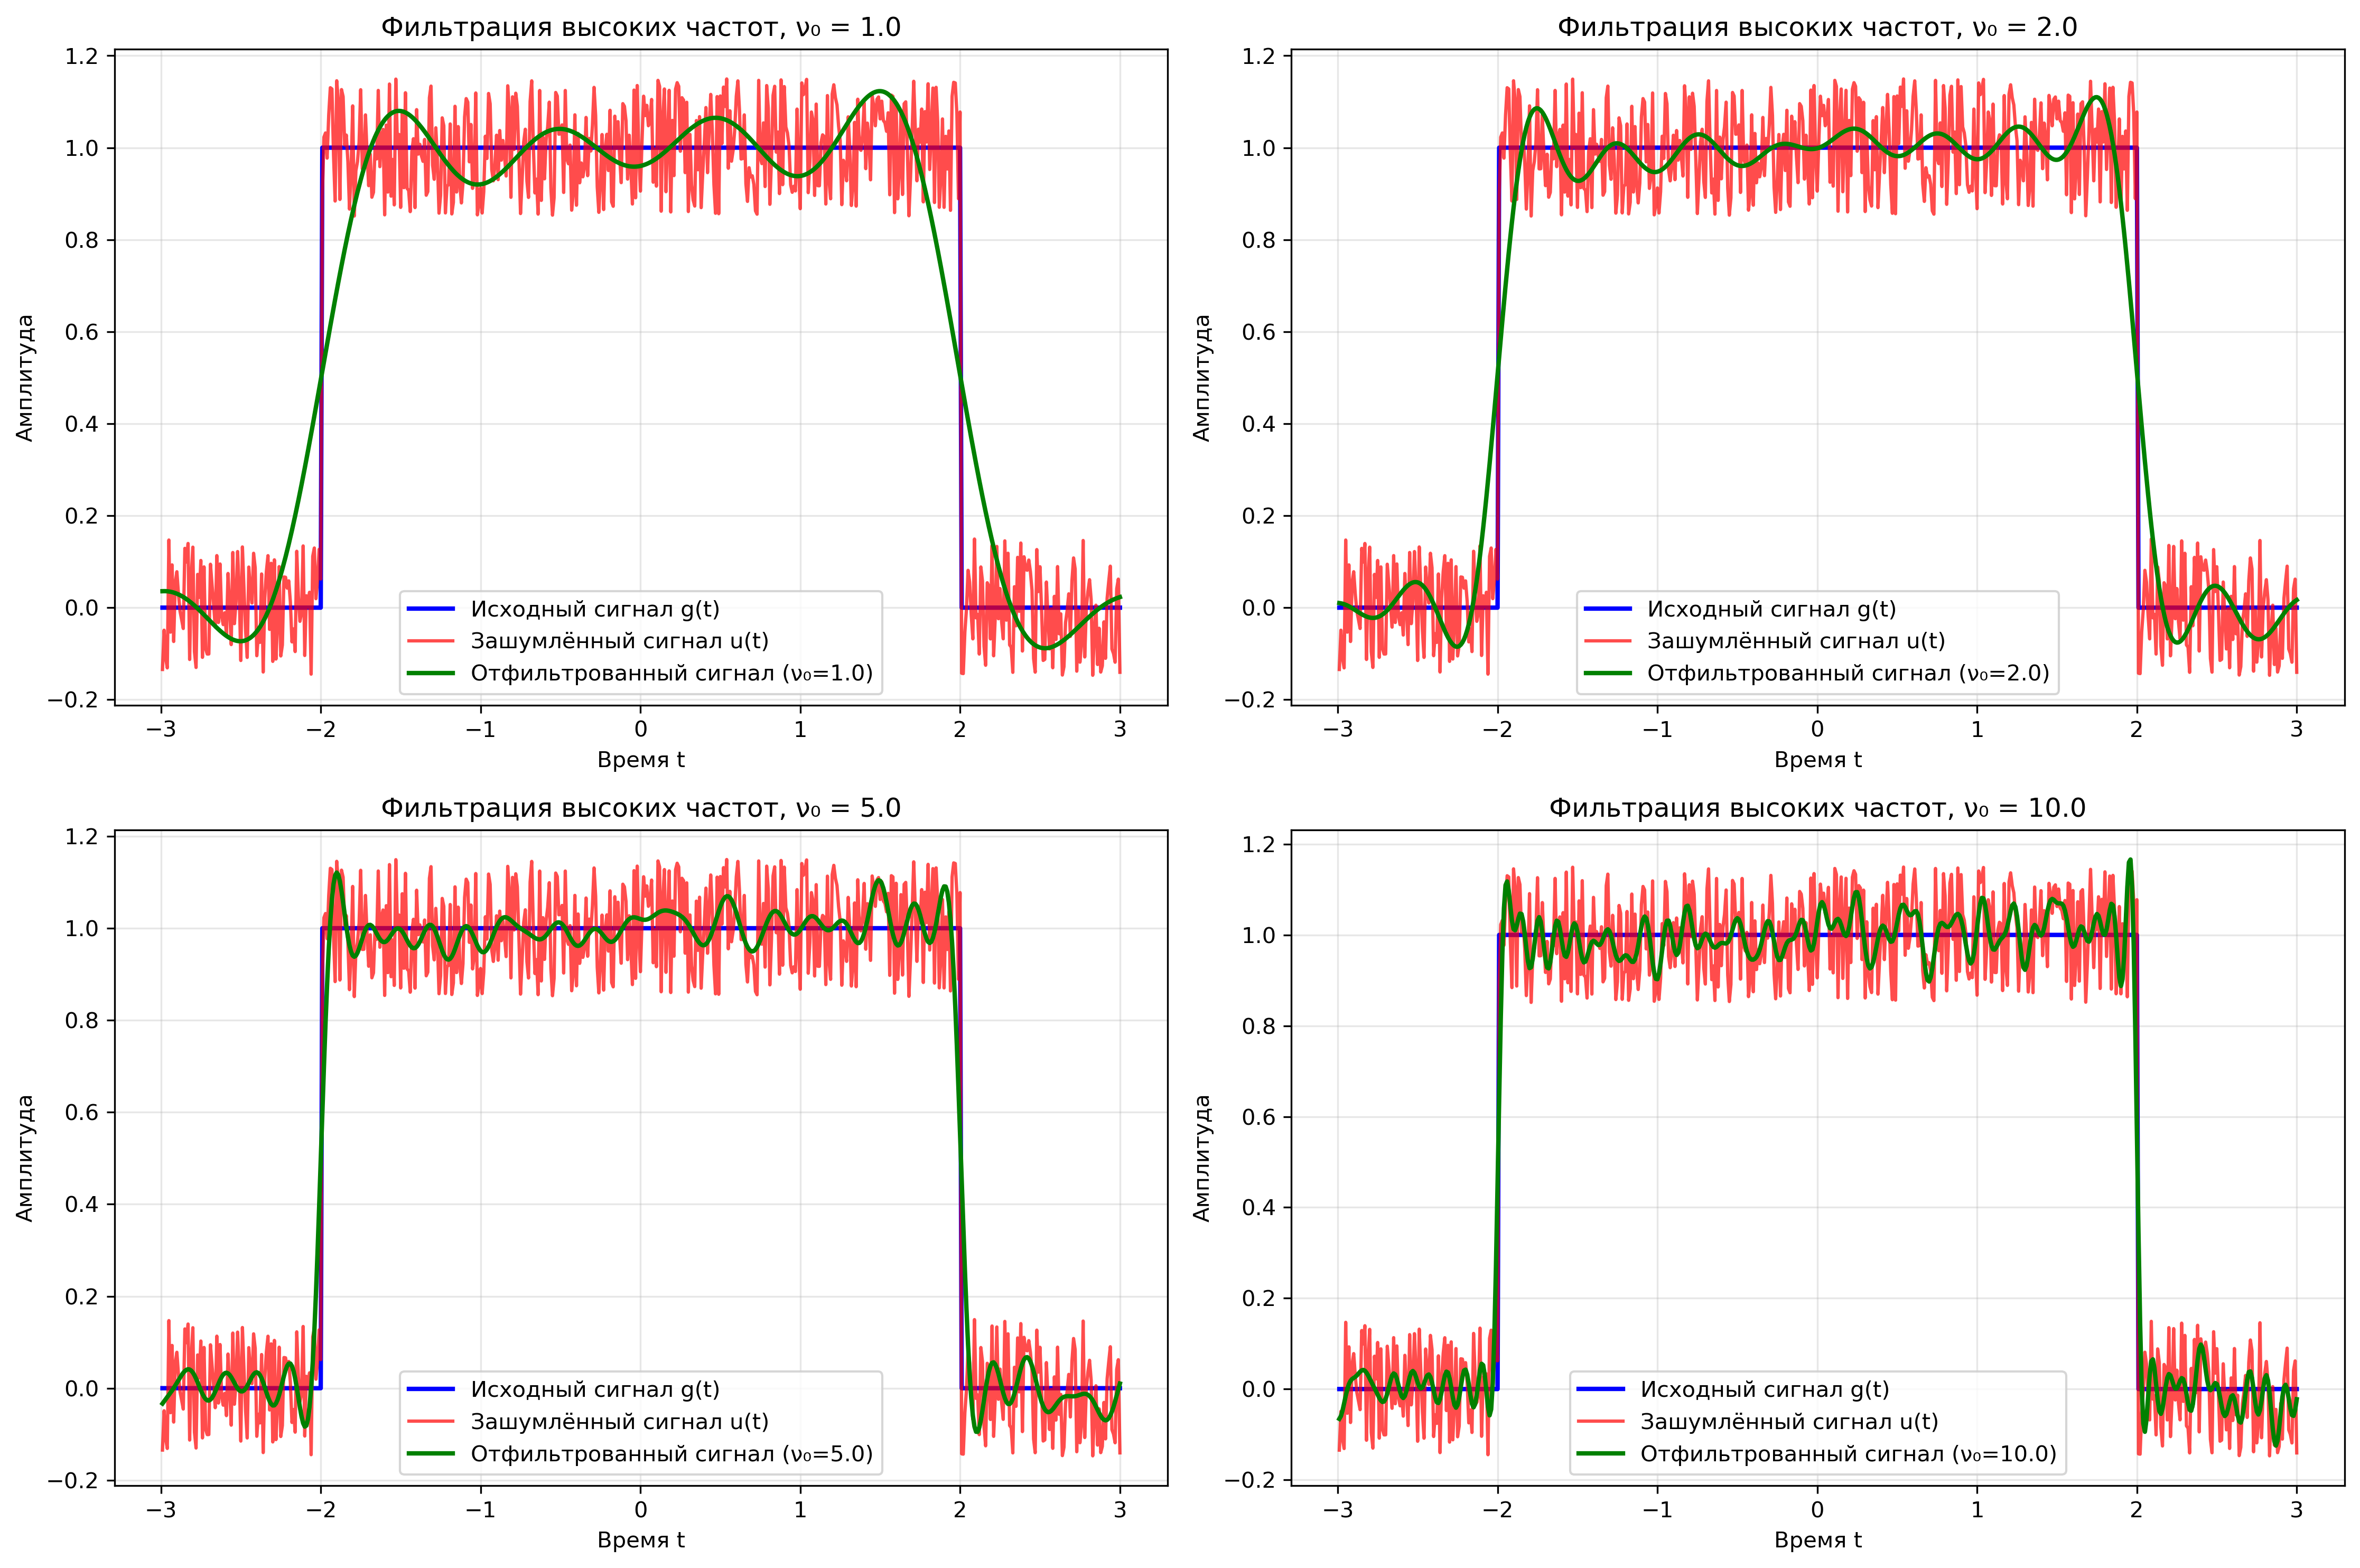
\includegraphics[width=\textwidth]{images/task1/high_freq_filter_time_domain.png}
\caption{Сравнение сигналов во временной области при фильтрации высоких частот}
\end{figure}

\begin{figure}[H]
\centering
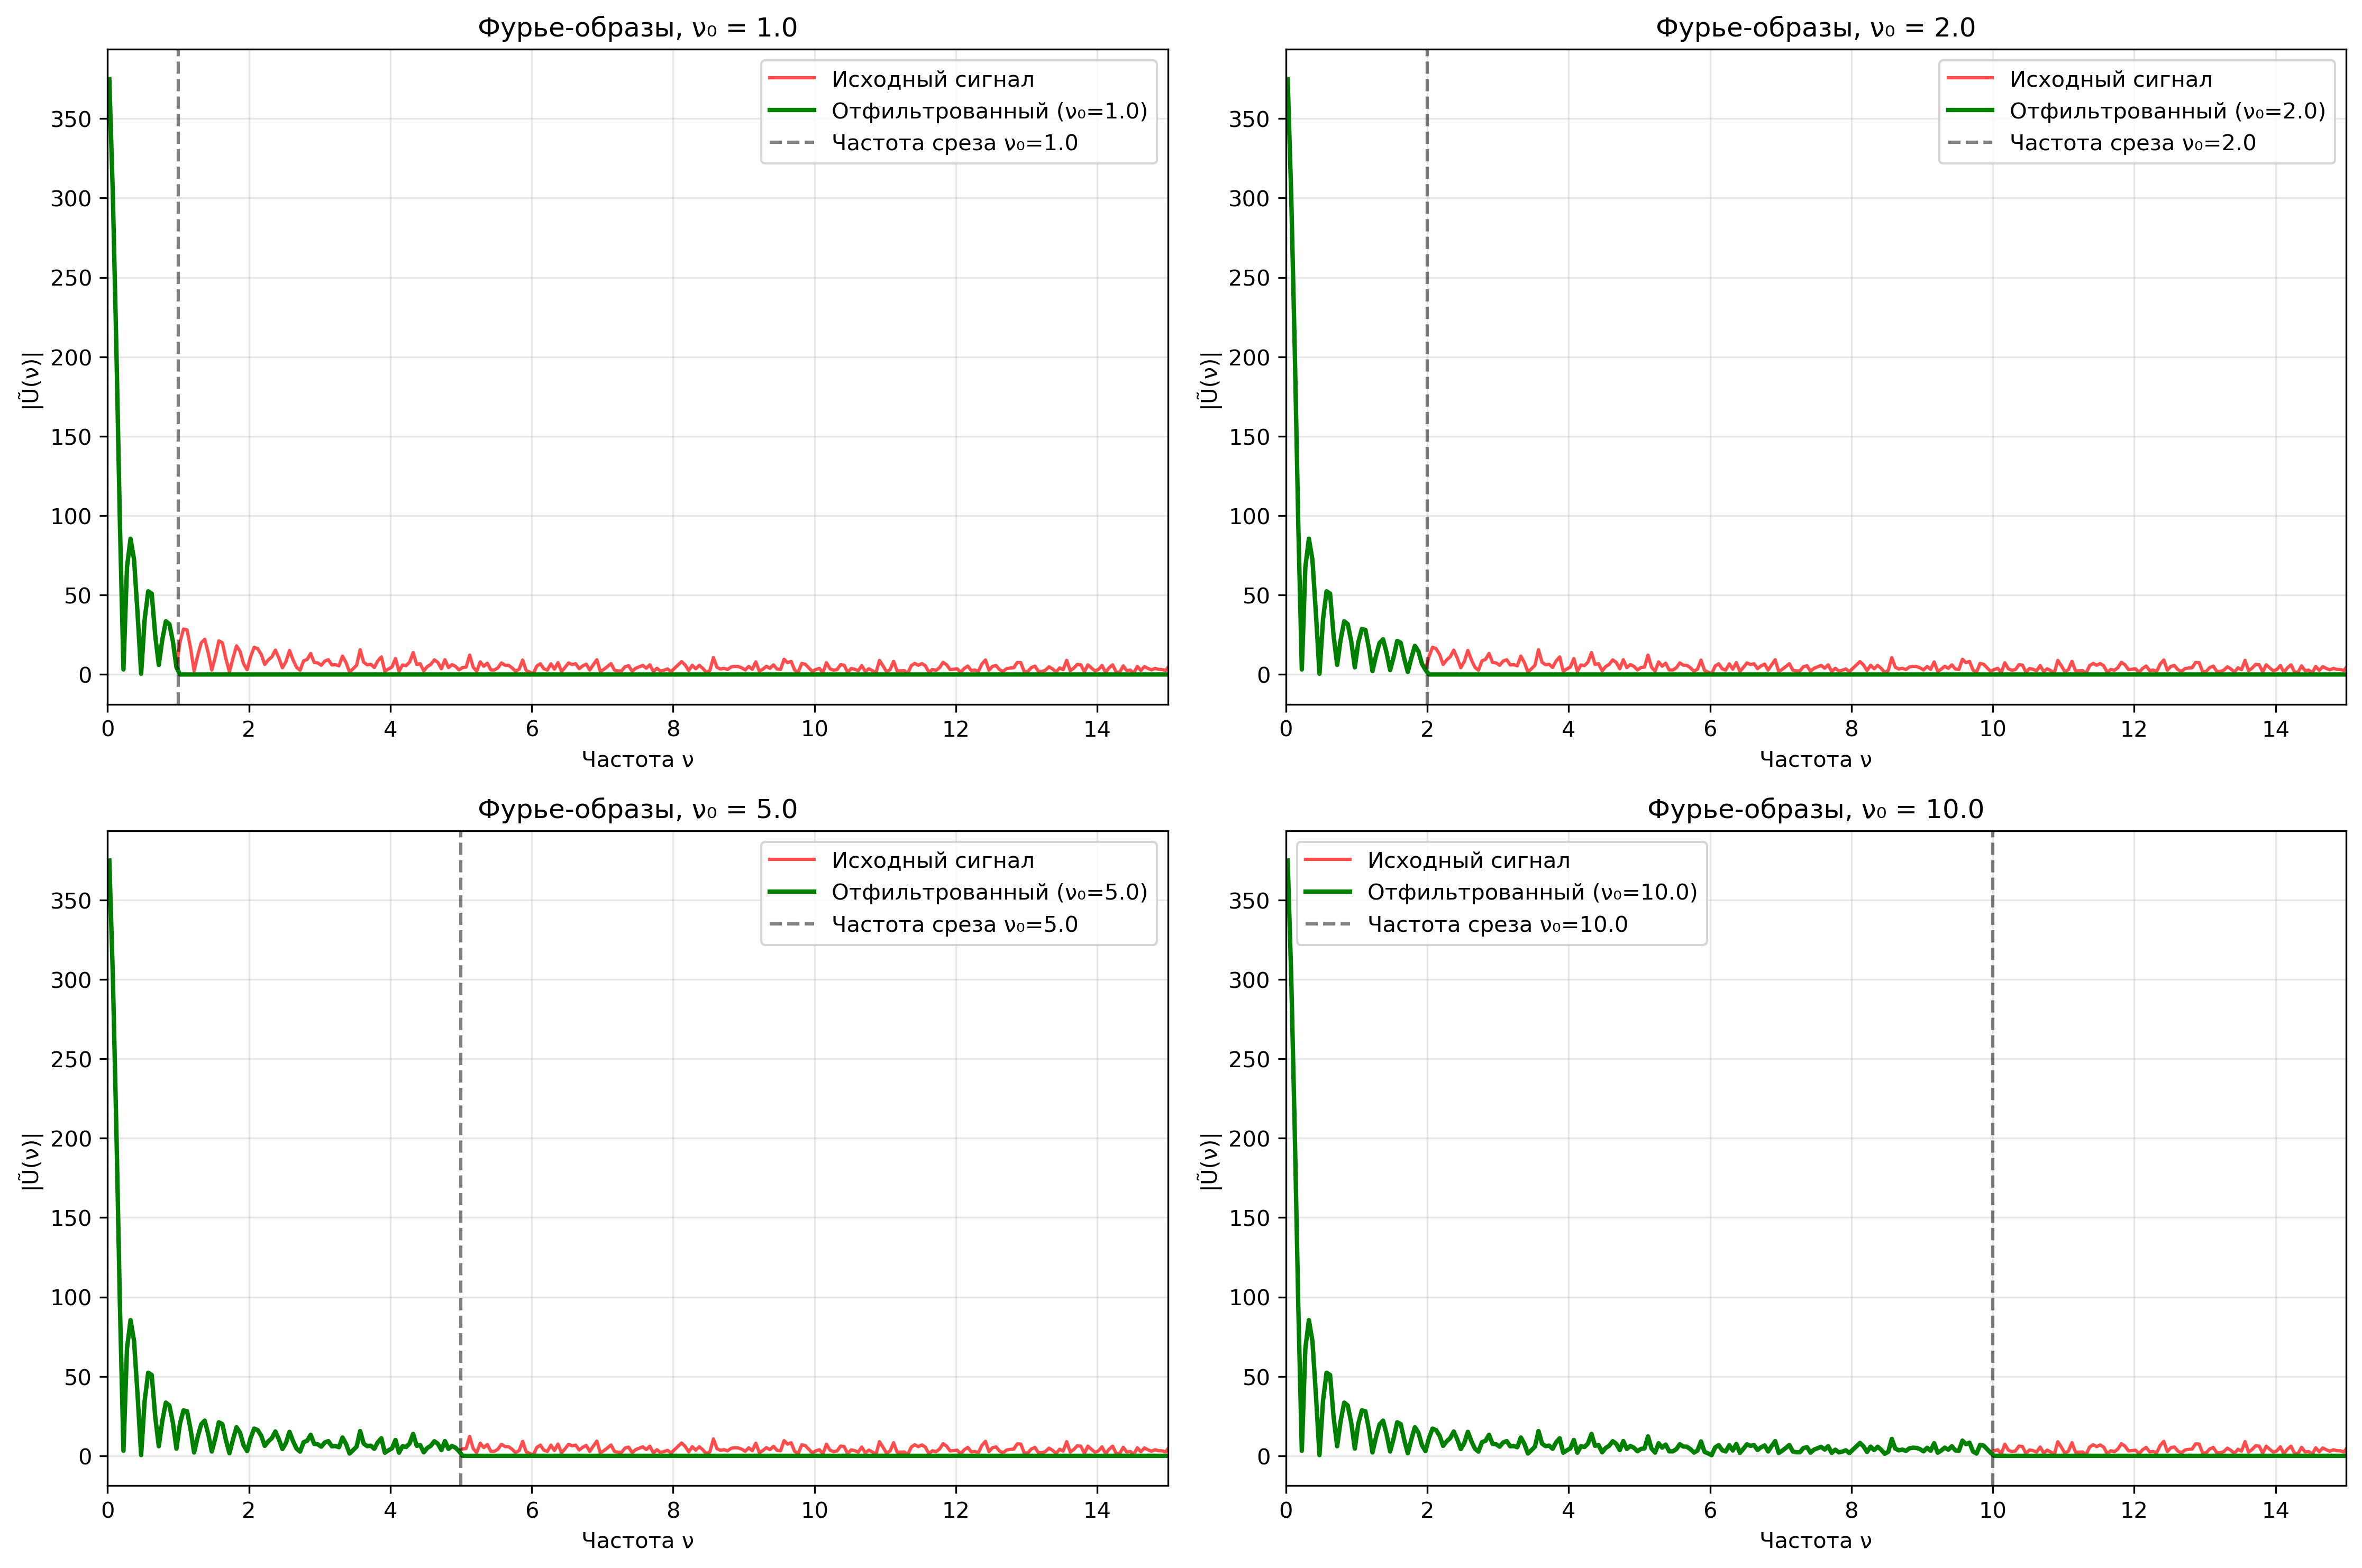
\includegraphics[width=\textwidth]{images/task1/high_freq_filter_freq_domain.png}
\caption{Сравнение Фурье-образов при фильтрации высоких частот}
\end{figure}

\begin{figure}[H]
\centering
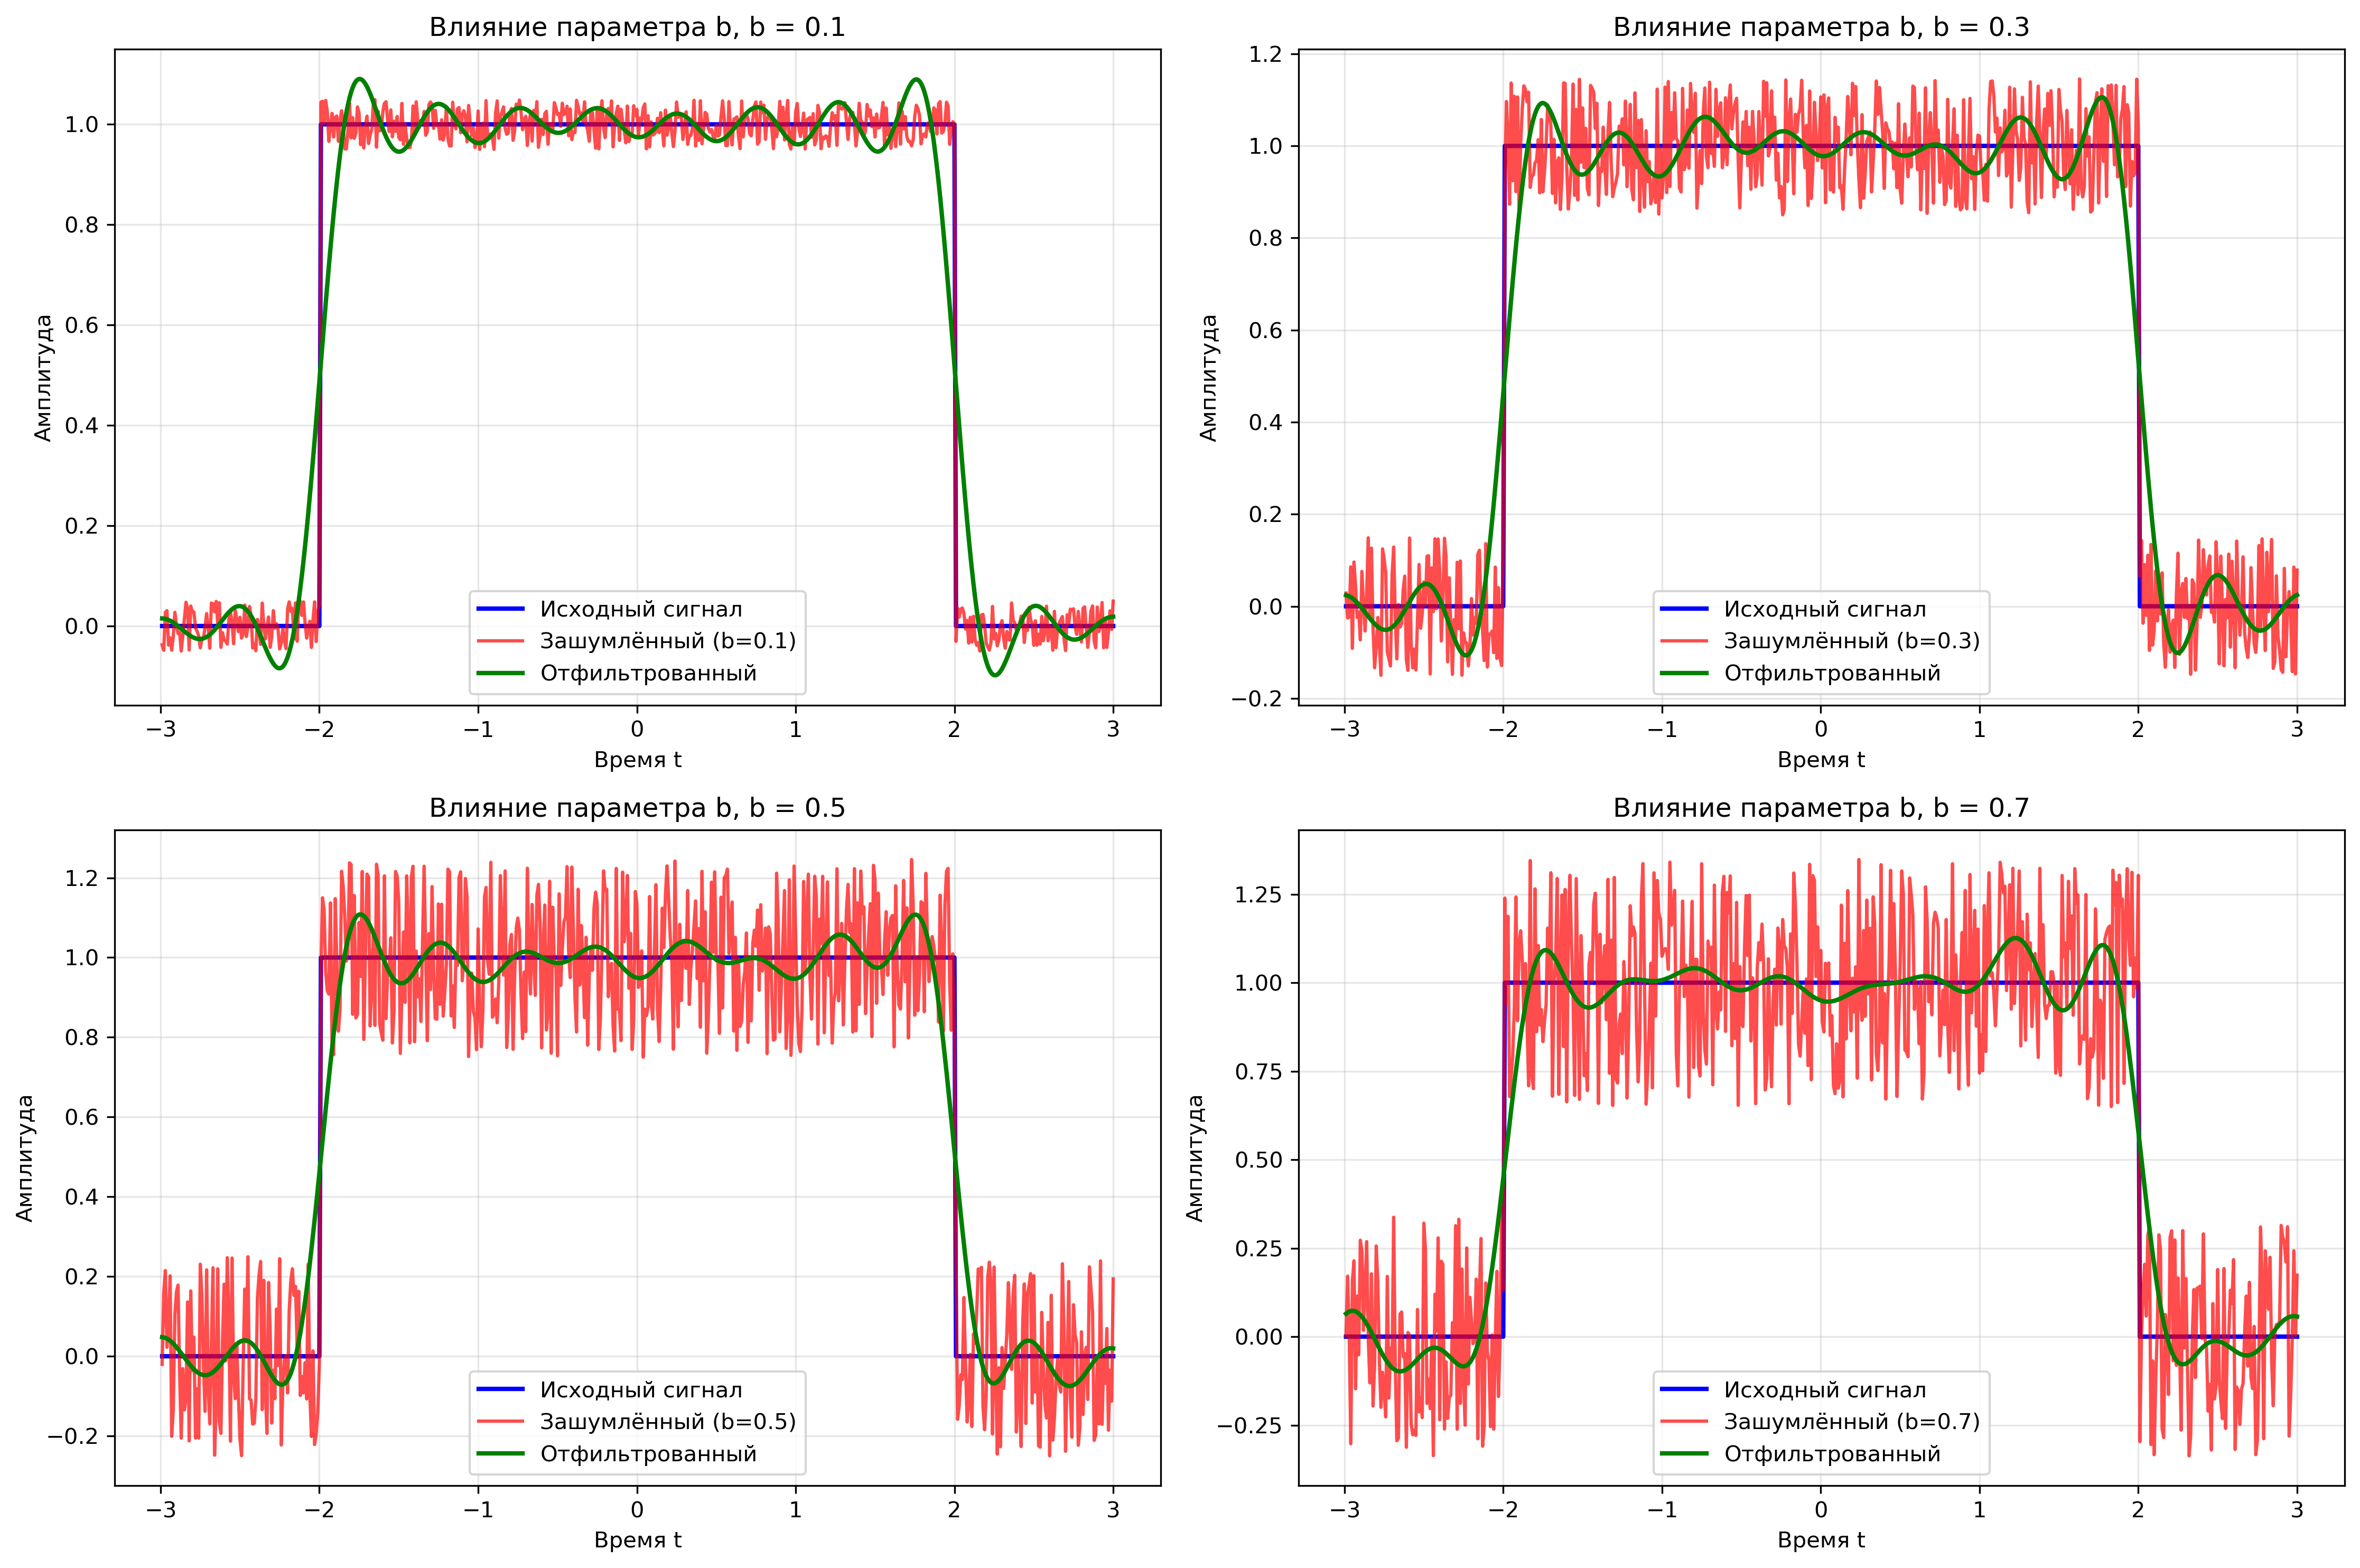
\includegraphics[width=\textwidth]{images/task1/high_freq_filter_b_influence.png}
\caption{Влияние параметра b на эффективность фильтрации высоких частот}
\end{figure}

\textbf{Анализ результатов:}

При фильтрации высоких частот наблюдаются следующие эффекты:

\begin{itemize}
    \item \textbf{Влияние частоты среза $v_0$:} При малых значениях $v_0$ (1-2 Гц) фильтрация недостаточно эффективна, так как сохраняется много шума. При больших значениях (5-10 Гц) качество фильтрации улучшается, но может происходить потеря полезной информации.
    
    \item \textbf{Влияние параметра b:} При увеличении амплитуды случайного шума (b) эффективность фильтрации снижается, так как шум становится более интенсивным и его сложнее отделить от полезного сигнала.
    
    \item \textbf{Оптимальная частота среза:} Для данных параметров оптимальной является частота среза $v_0$ = 2-5 Гц, которая обеспечивает хороший баланс между удалением шума и сохранением формы исходного сигнала.
\end{itemize}

\subsection*{Фильтрация специфических частот}

В данном разделе исследуется фильтрация при ненулевых параметрах $b, c, d$.

\textbf{Дополнительные параметры:}
\begin{itemize}
    \item $c = 0.5$ — амплитуда гармонической помехи
    \item $d = 10.0$ — частота гармонической помехи
\end{itemize}

\textbf{Метод фильтрации:}
\begin{itemize}
    \item Обнуляем Фурье-образ на диапазонах частот, соответствующих помехам
    \item Убираем влияние как случайного шума, так и гармонической помехи
    \item Исследуем влияние частот среза и параметров $b, c, d$ на эффективность
\end{itemize}

\begin{figure}[H]
\centering
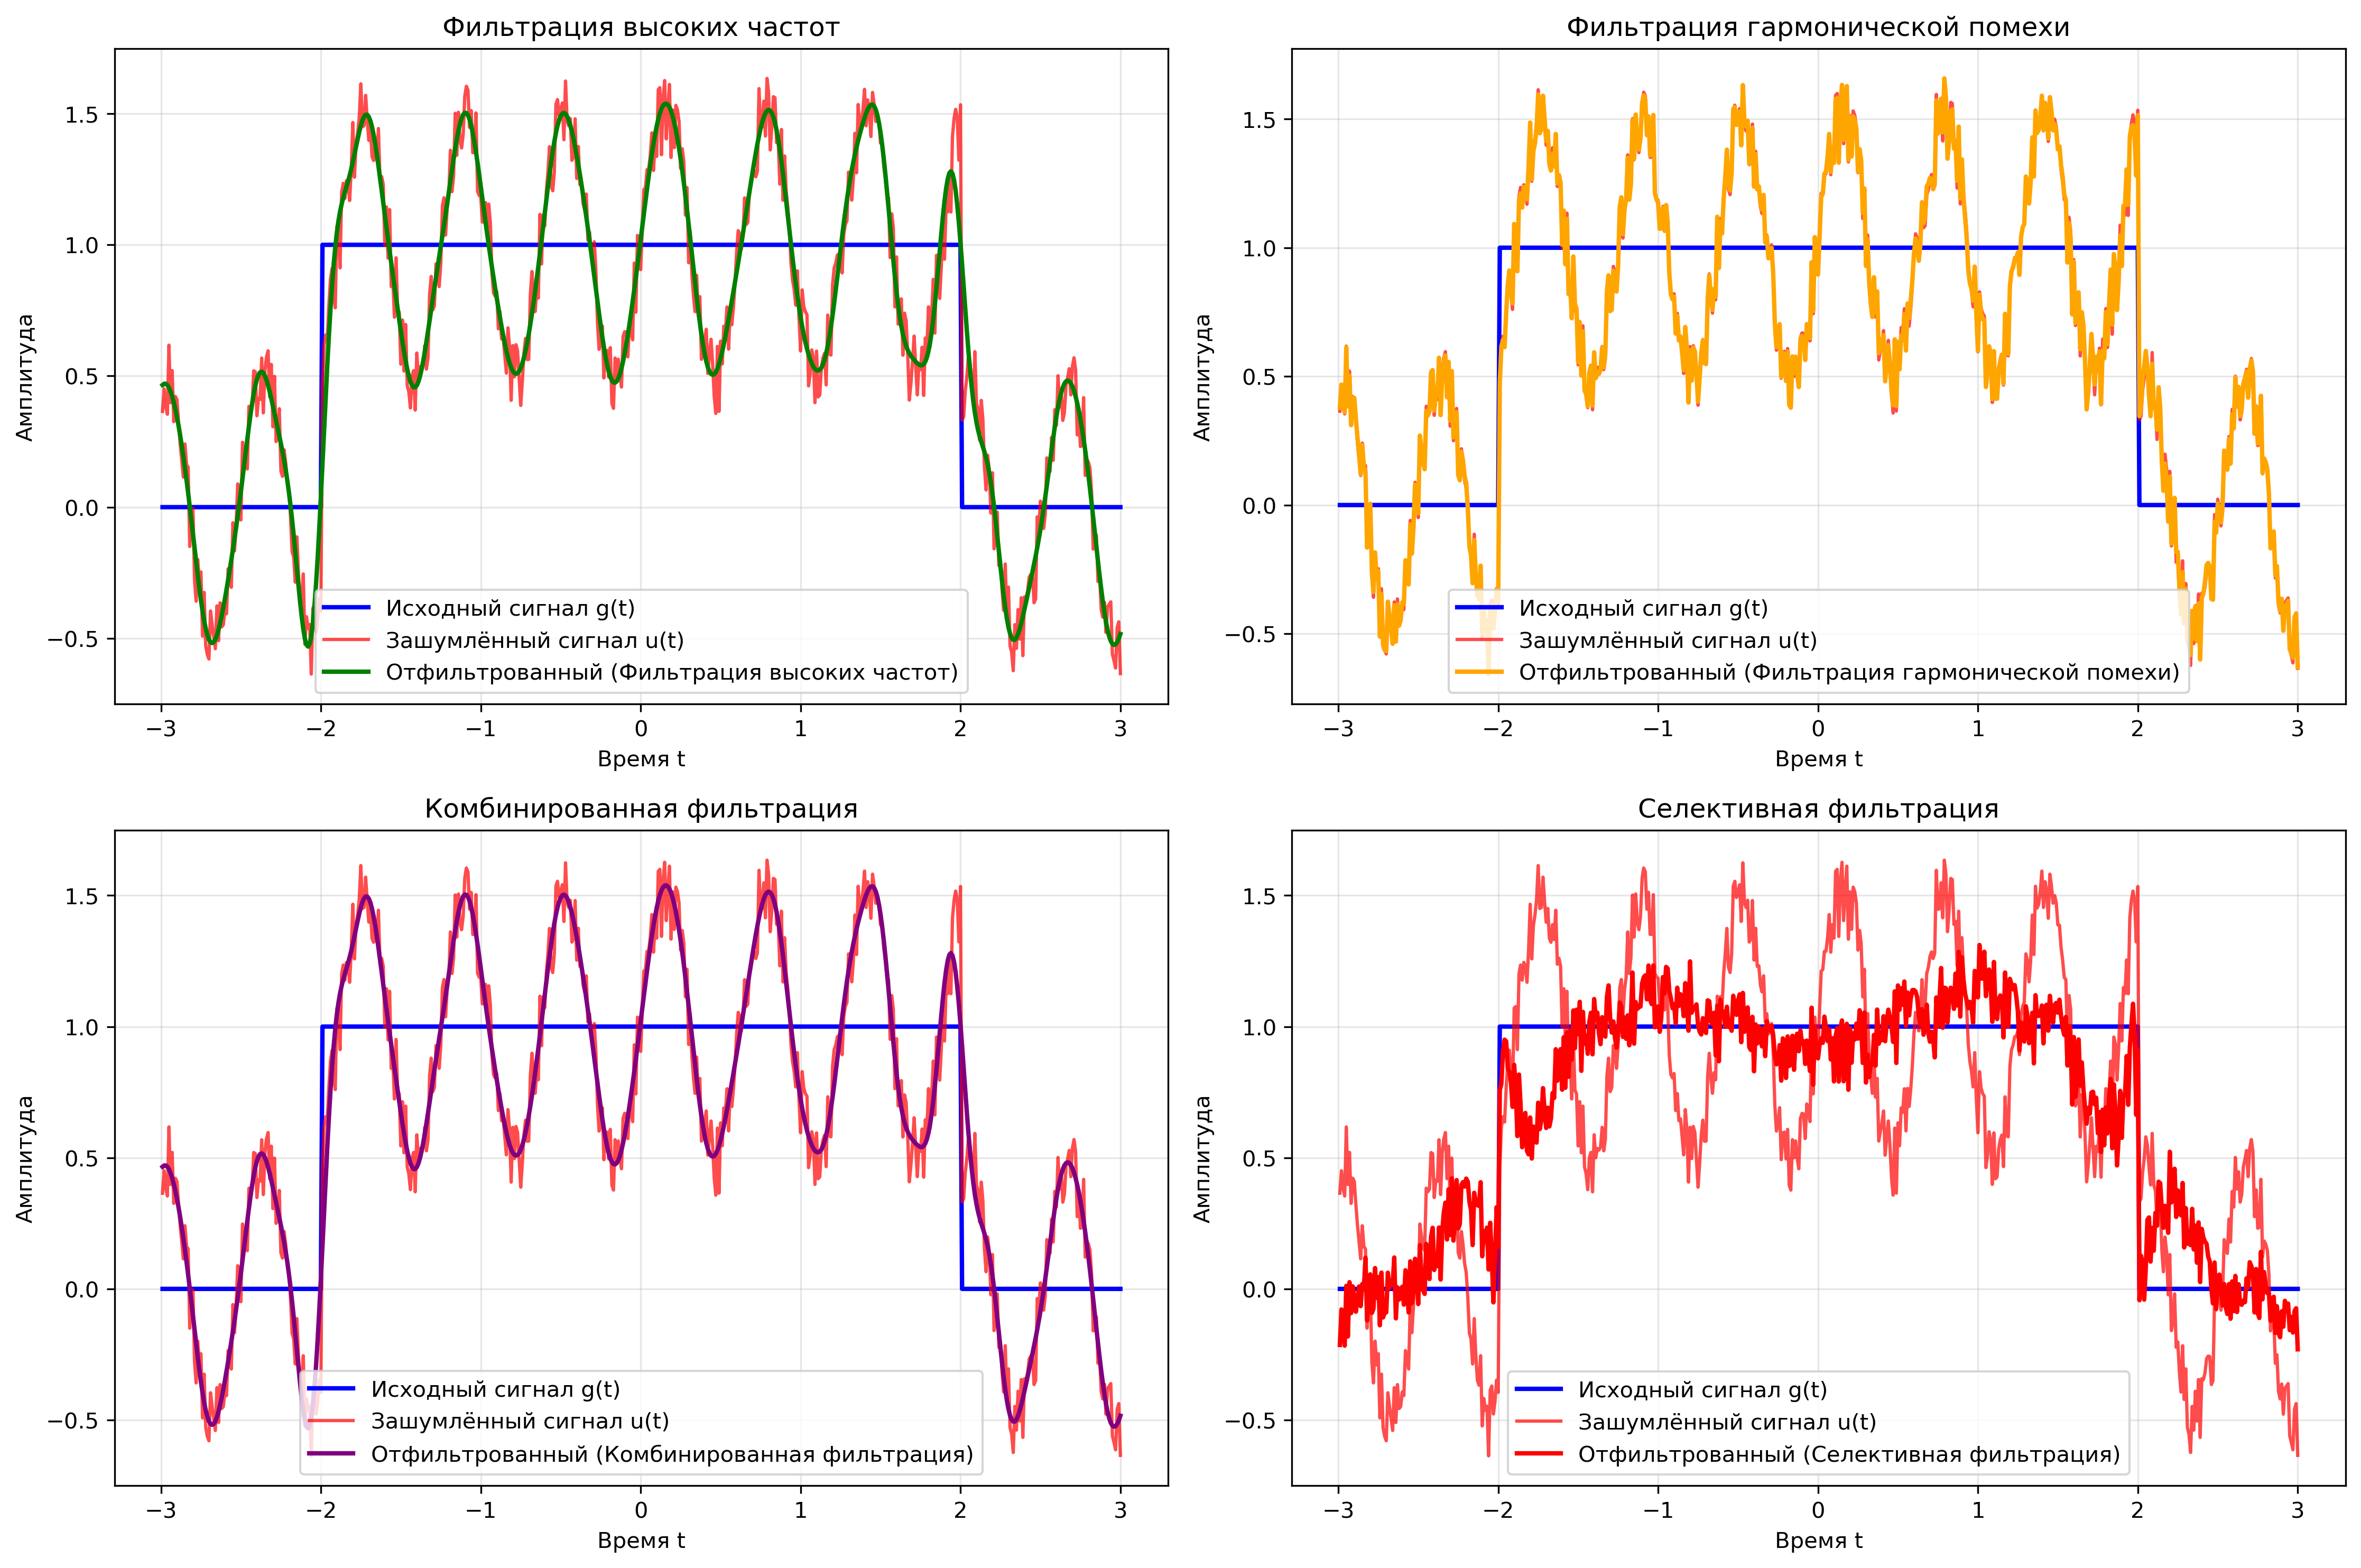
\includegraphics[width=\textwidth]{images/task1/specific_freq_filter_time_domain.png}
\caption{Сравнение сигналов во временной области при фильтрации специфических частот}
\end{figure}

\begin{figure}[H]
\centering
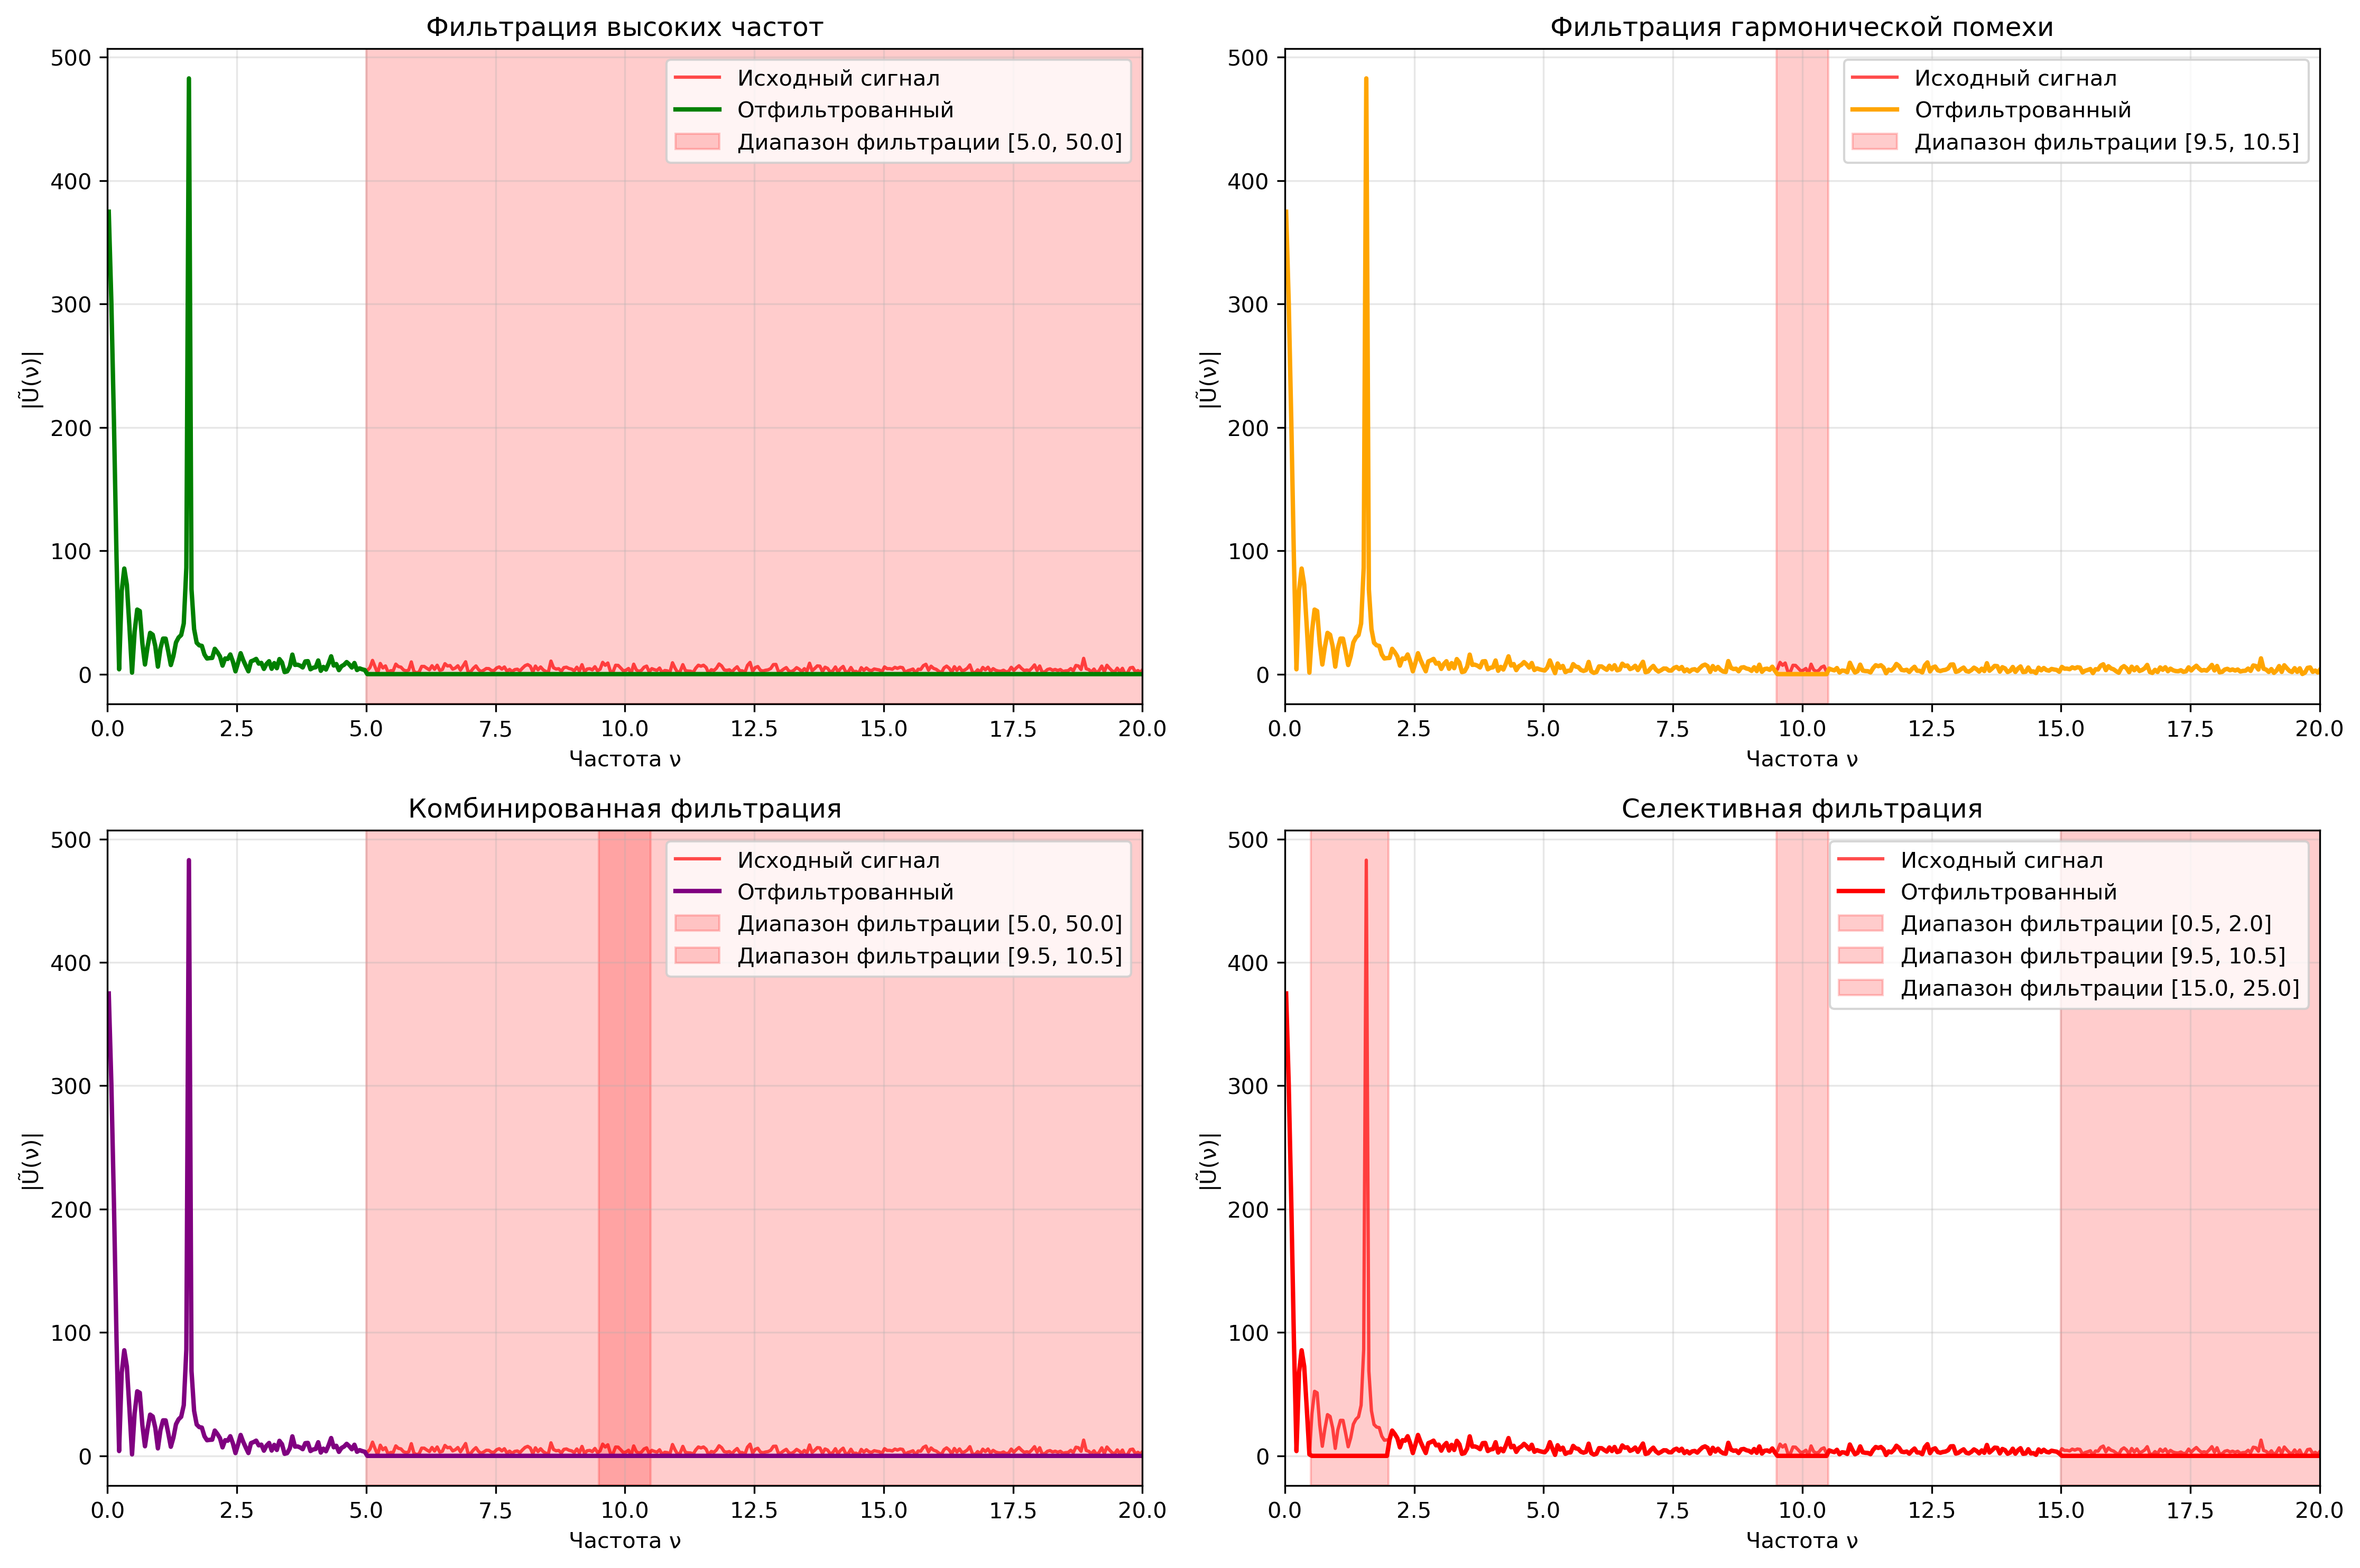
\includegraphics[width=\textwidth]{images/task1/specific_freq_filter_freq_domain.png}
\caption{Сравнение Фурье-образов при фильтрации специфических частот}
\end{figure}

\begin{figure}[H]
\centering
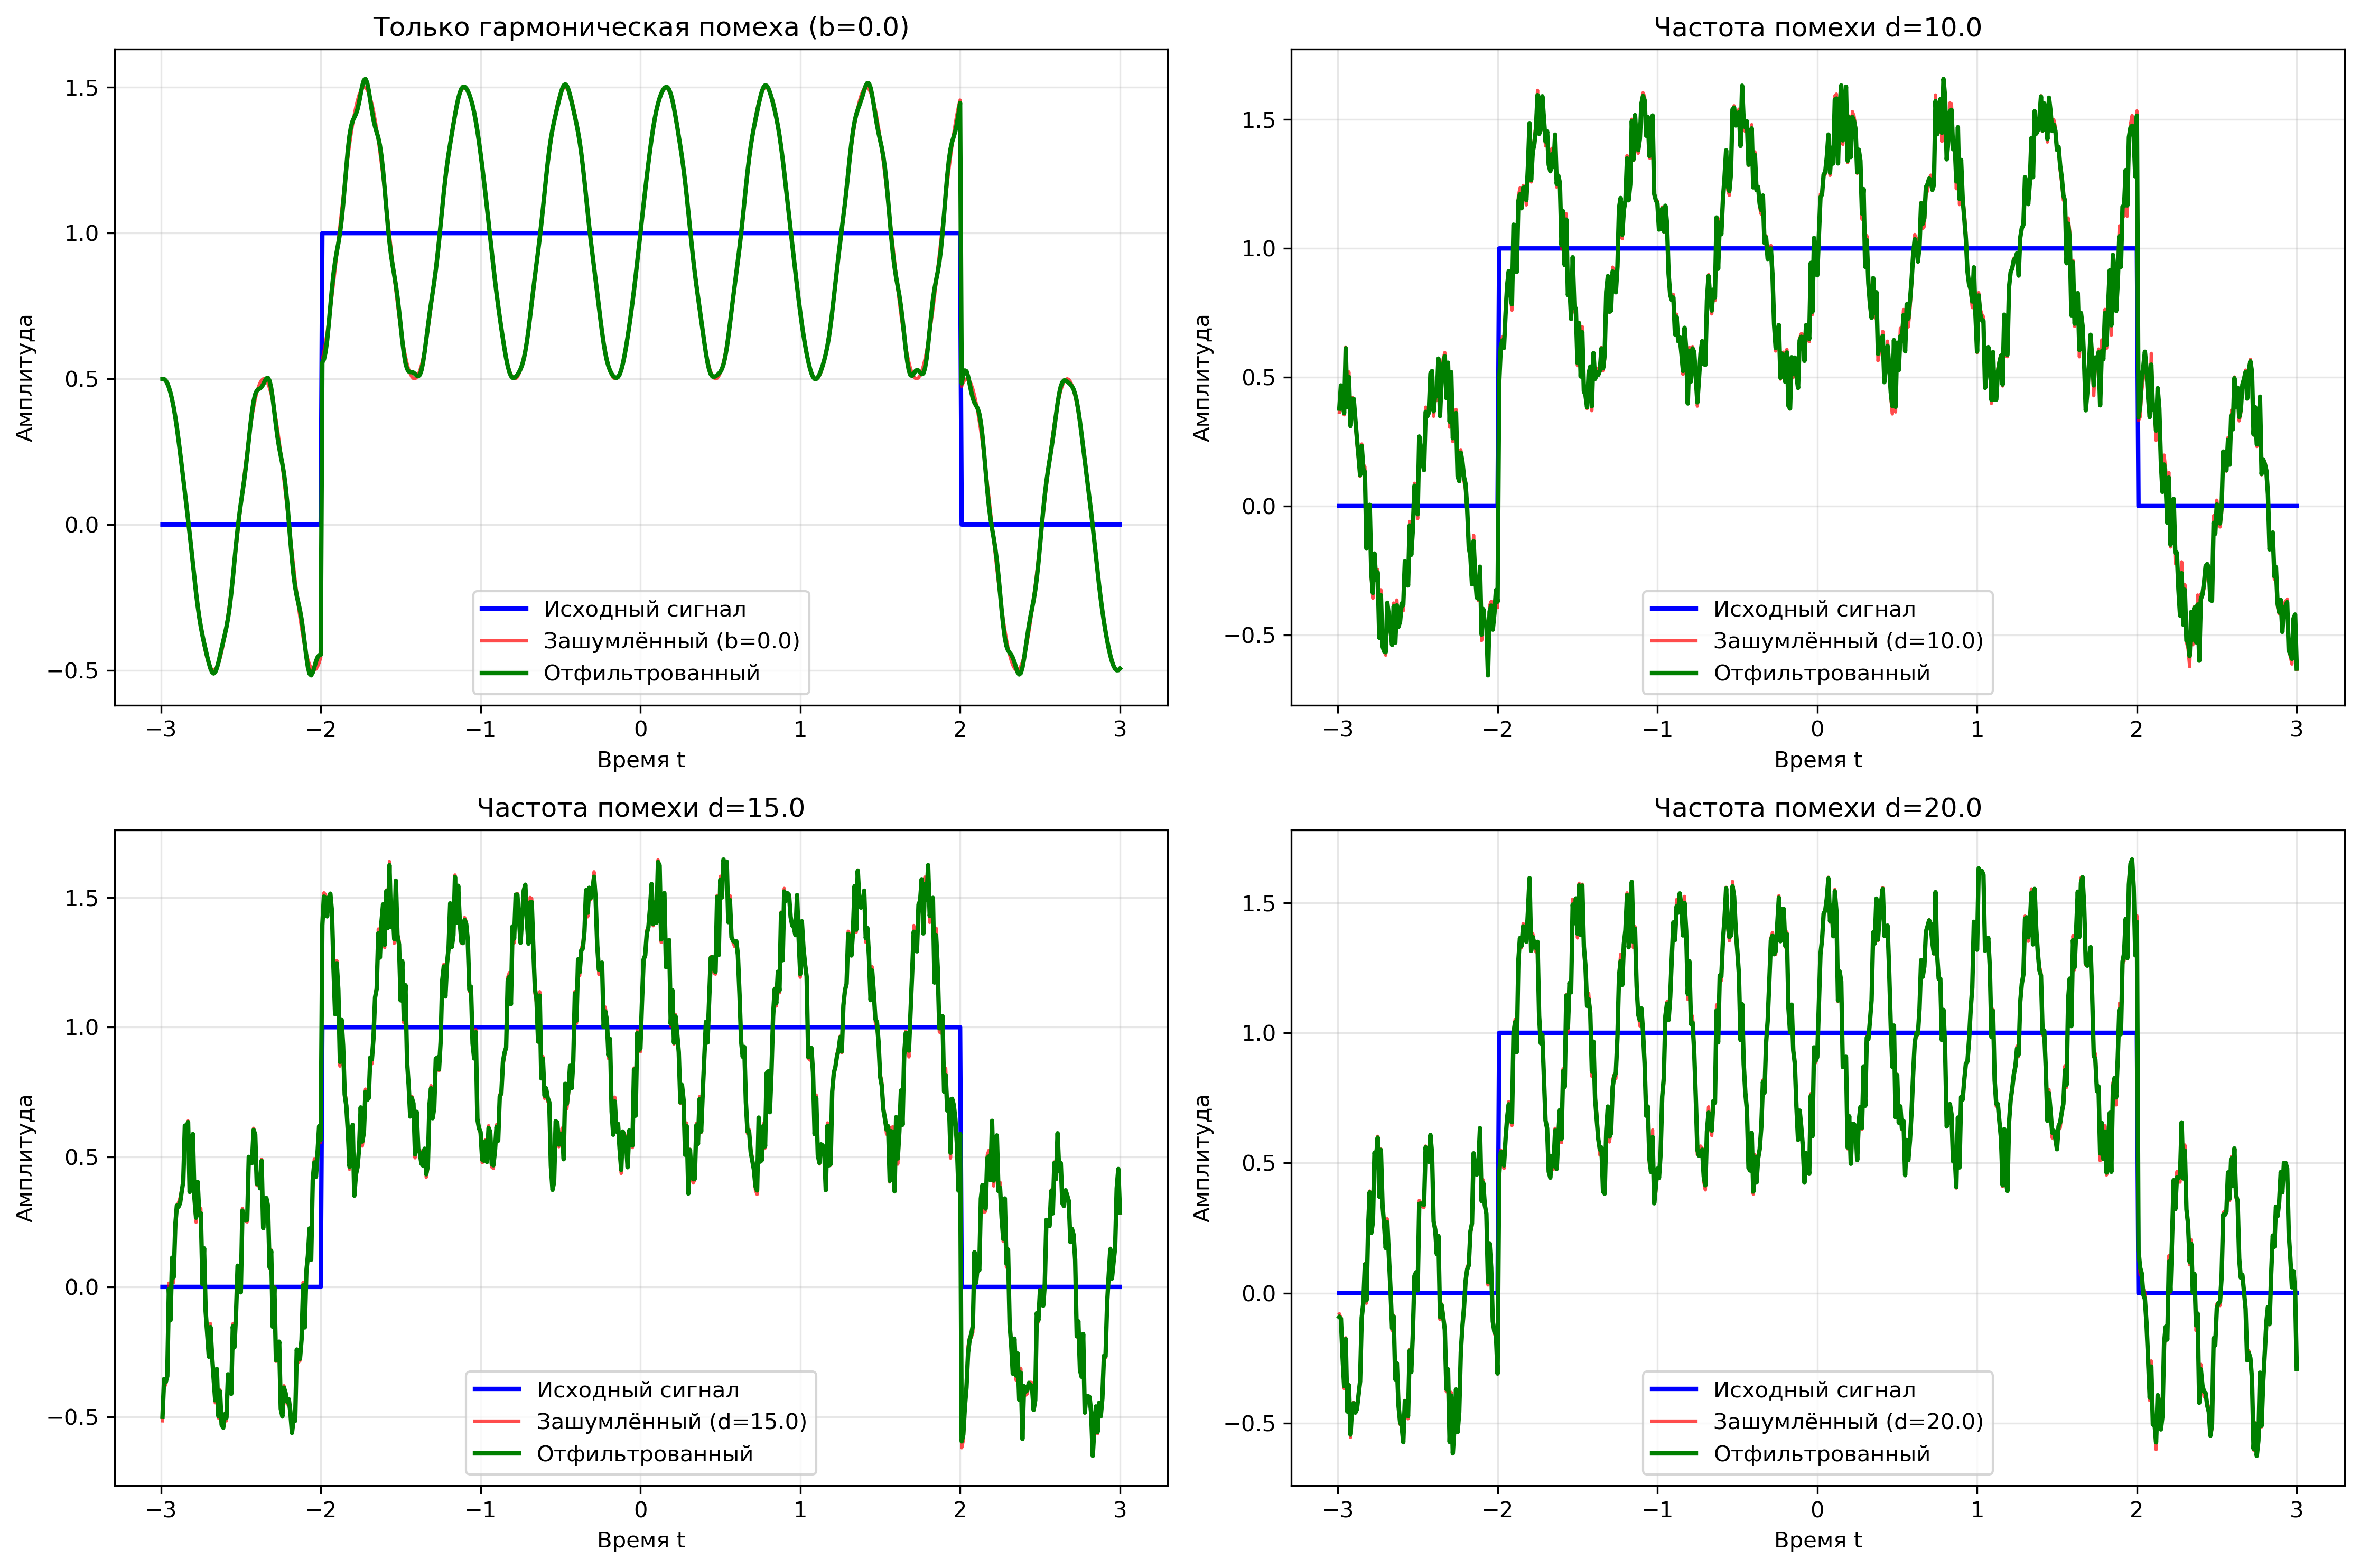
\includegraphics[width=\textwidth]{images/task1/specific_freq_filter_parameters.png}
\caption{Влияние параметров b, c, d на эффективность фильтрации}
\end{figure}

\textbf{Анализ результатов:}

При фильтрации специфических частот наблюдаются следующие эффекты:

\begin{itemize}
    \item \textbf{Фильтрация высоких частот:} Эффективно удаляет случайный шум, но может не справляться с гармоническими помехами.
    
    \item \textbf{Фильтрация гармонической помехи:} Точно удаляет помеху на частоте d = 10 Гц, но оставляет случайный шум.
    
    \item \textbf{Комбинированная фильтрация:} Наиболее эффективна, так как удаляет как случайный шум, так и гармонические помехи.
    
    \item \textbf{Селективная фильтрация:} Позволяет точно настроить диапазоны фильтрации под конкретные помехи.
\end{itemize}

\subsection*{Фильтрация низких частот}

Рассматривается фильтр, который обнуляет Фурье-образ на всех частотах в окрестности точки $\nu = 0$.

\textbf{Цель исследования:} оценить эффективность такого фильтра и его влияние на исходный сигнал.

\begin{figure}[H]
\centering
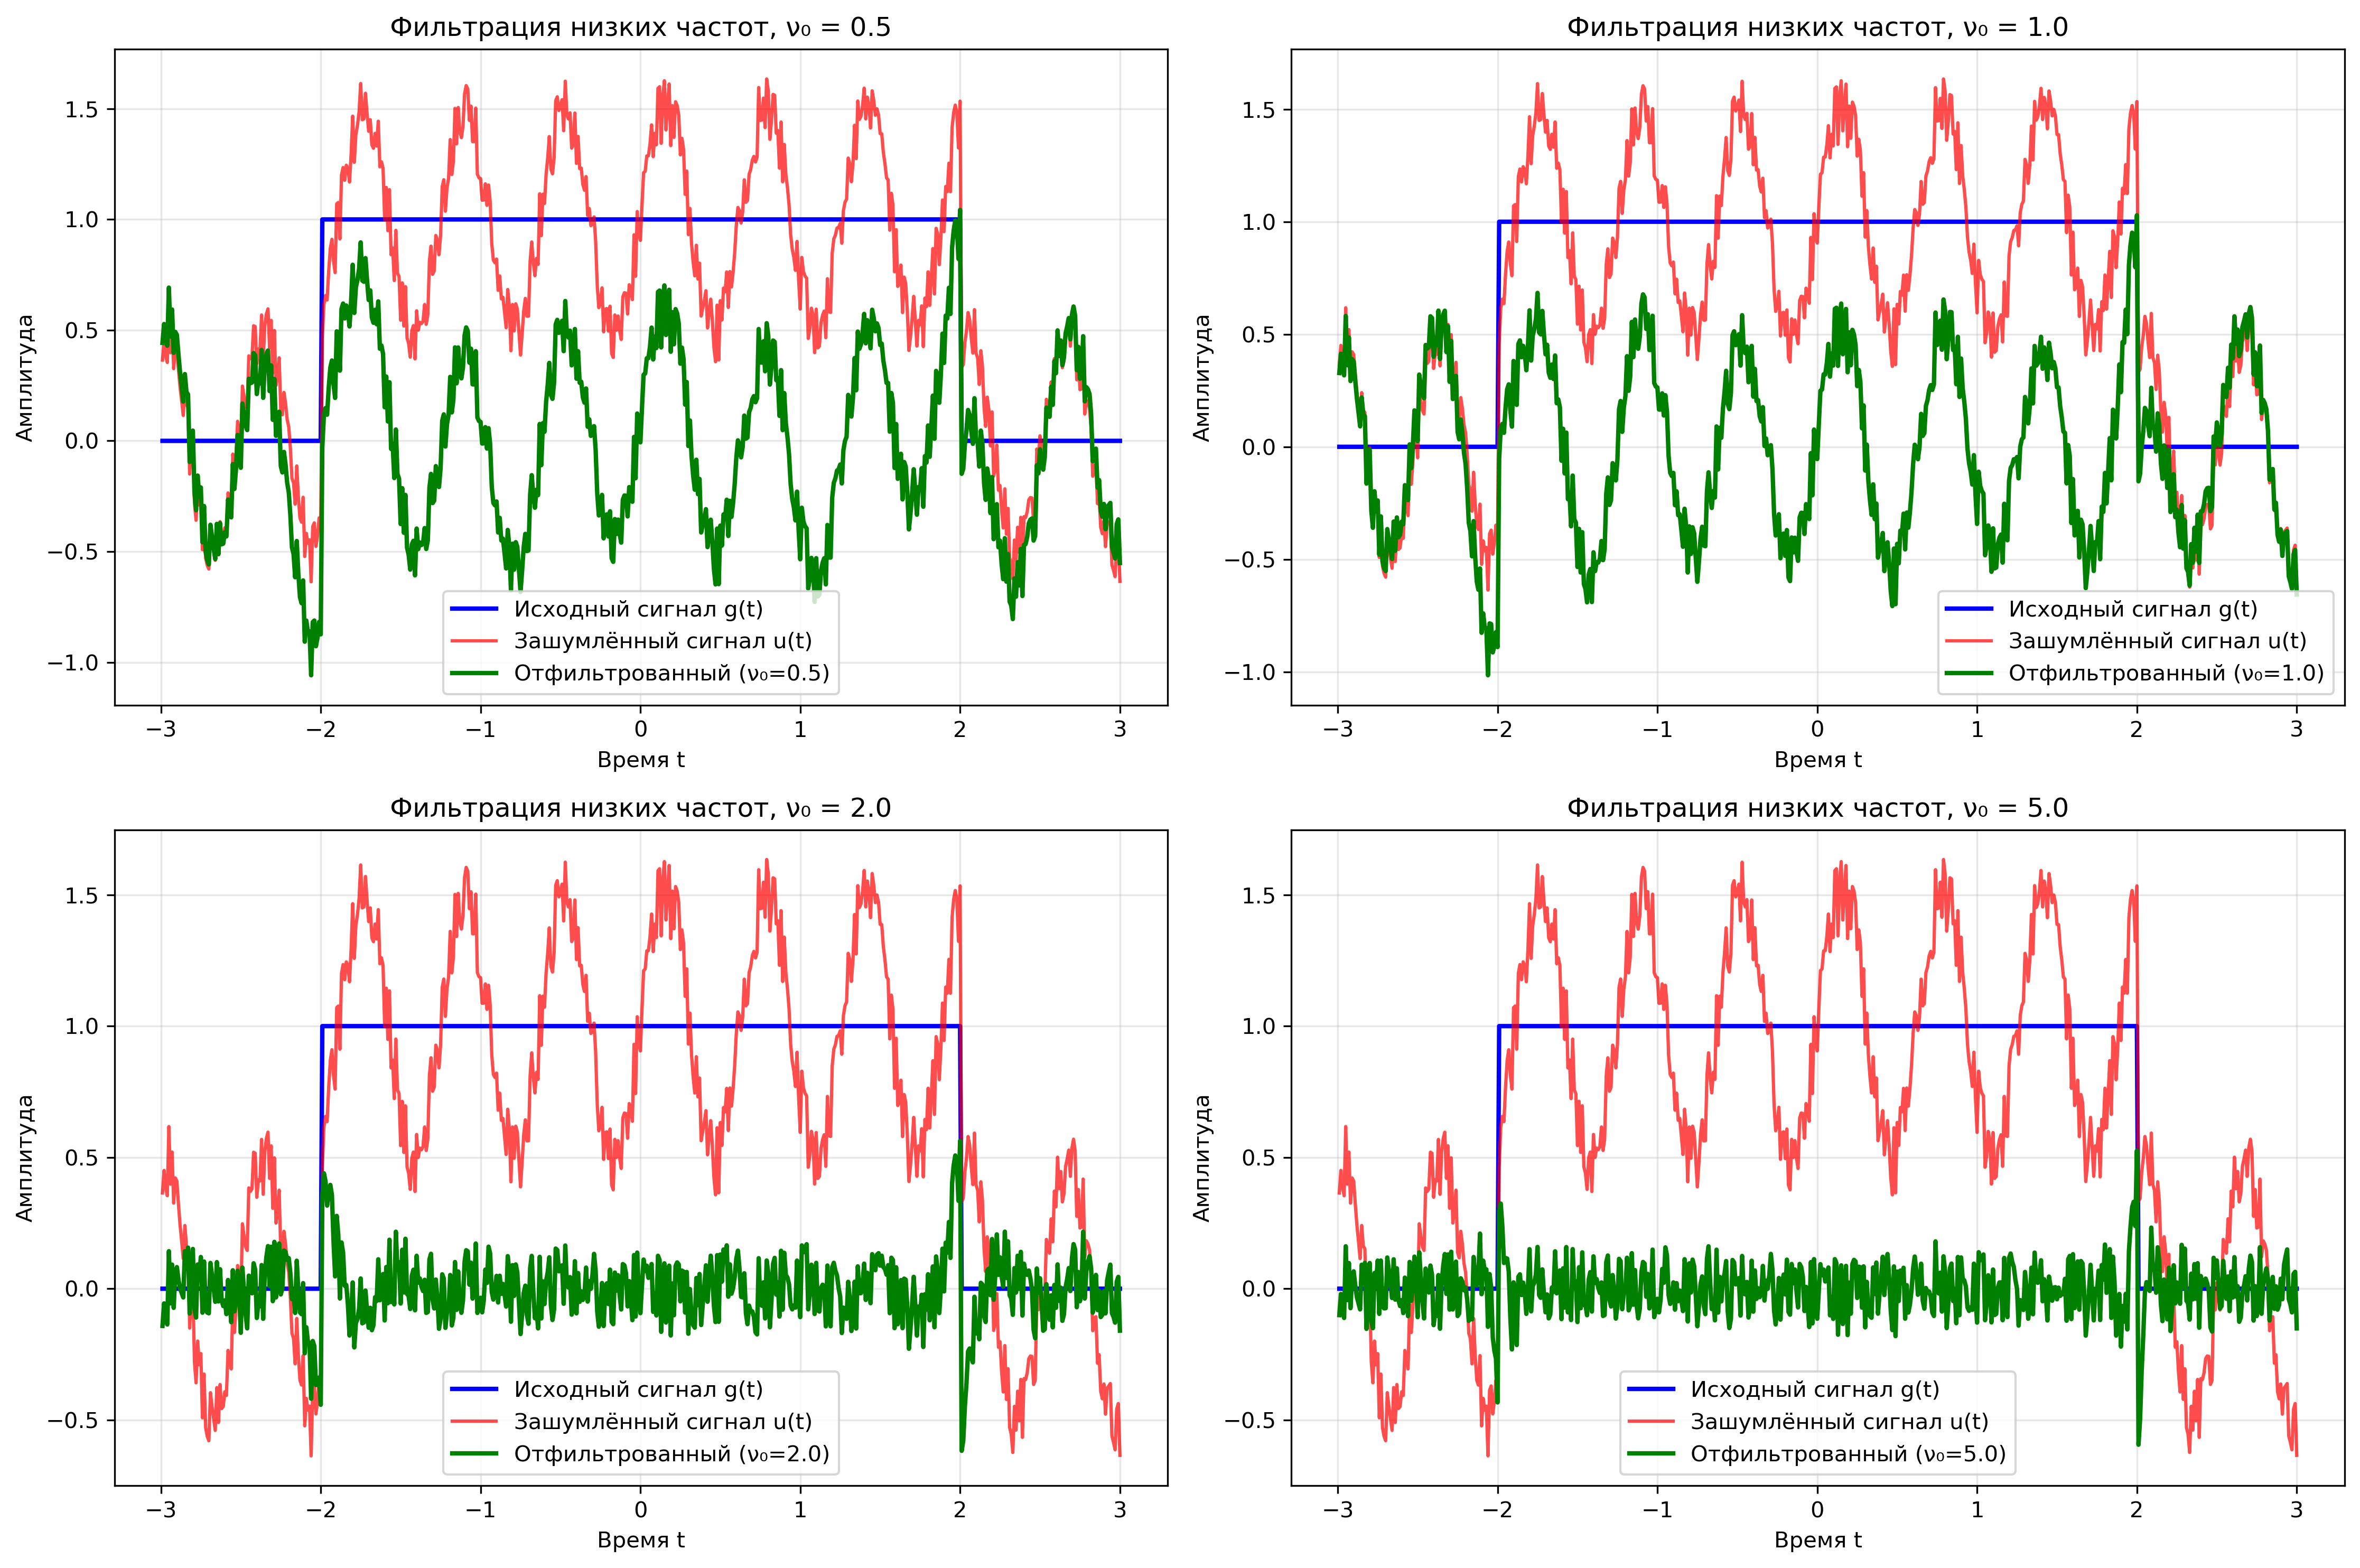
\includegraphics[width=\textwidth]{images/task1/low_freq_filter_time_domain.png}
\caption{Сравнение сигналов во временной области при фильтрации низких частот}
\end{figure}

\begin{figure}[H]
\centering
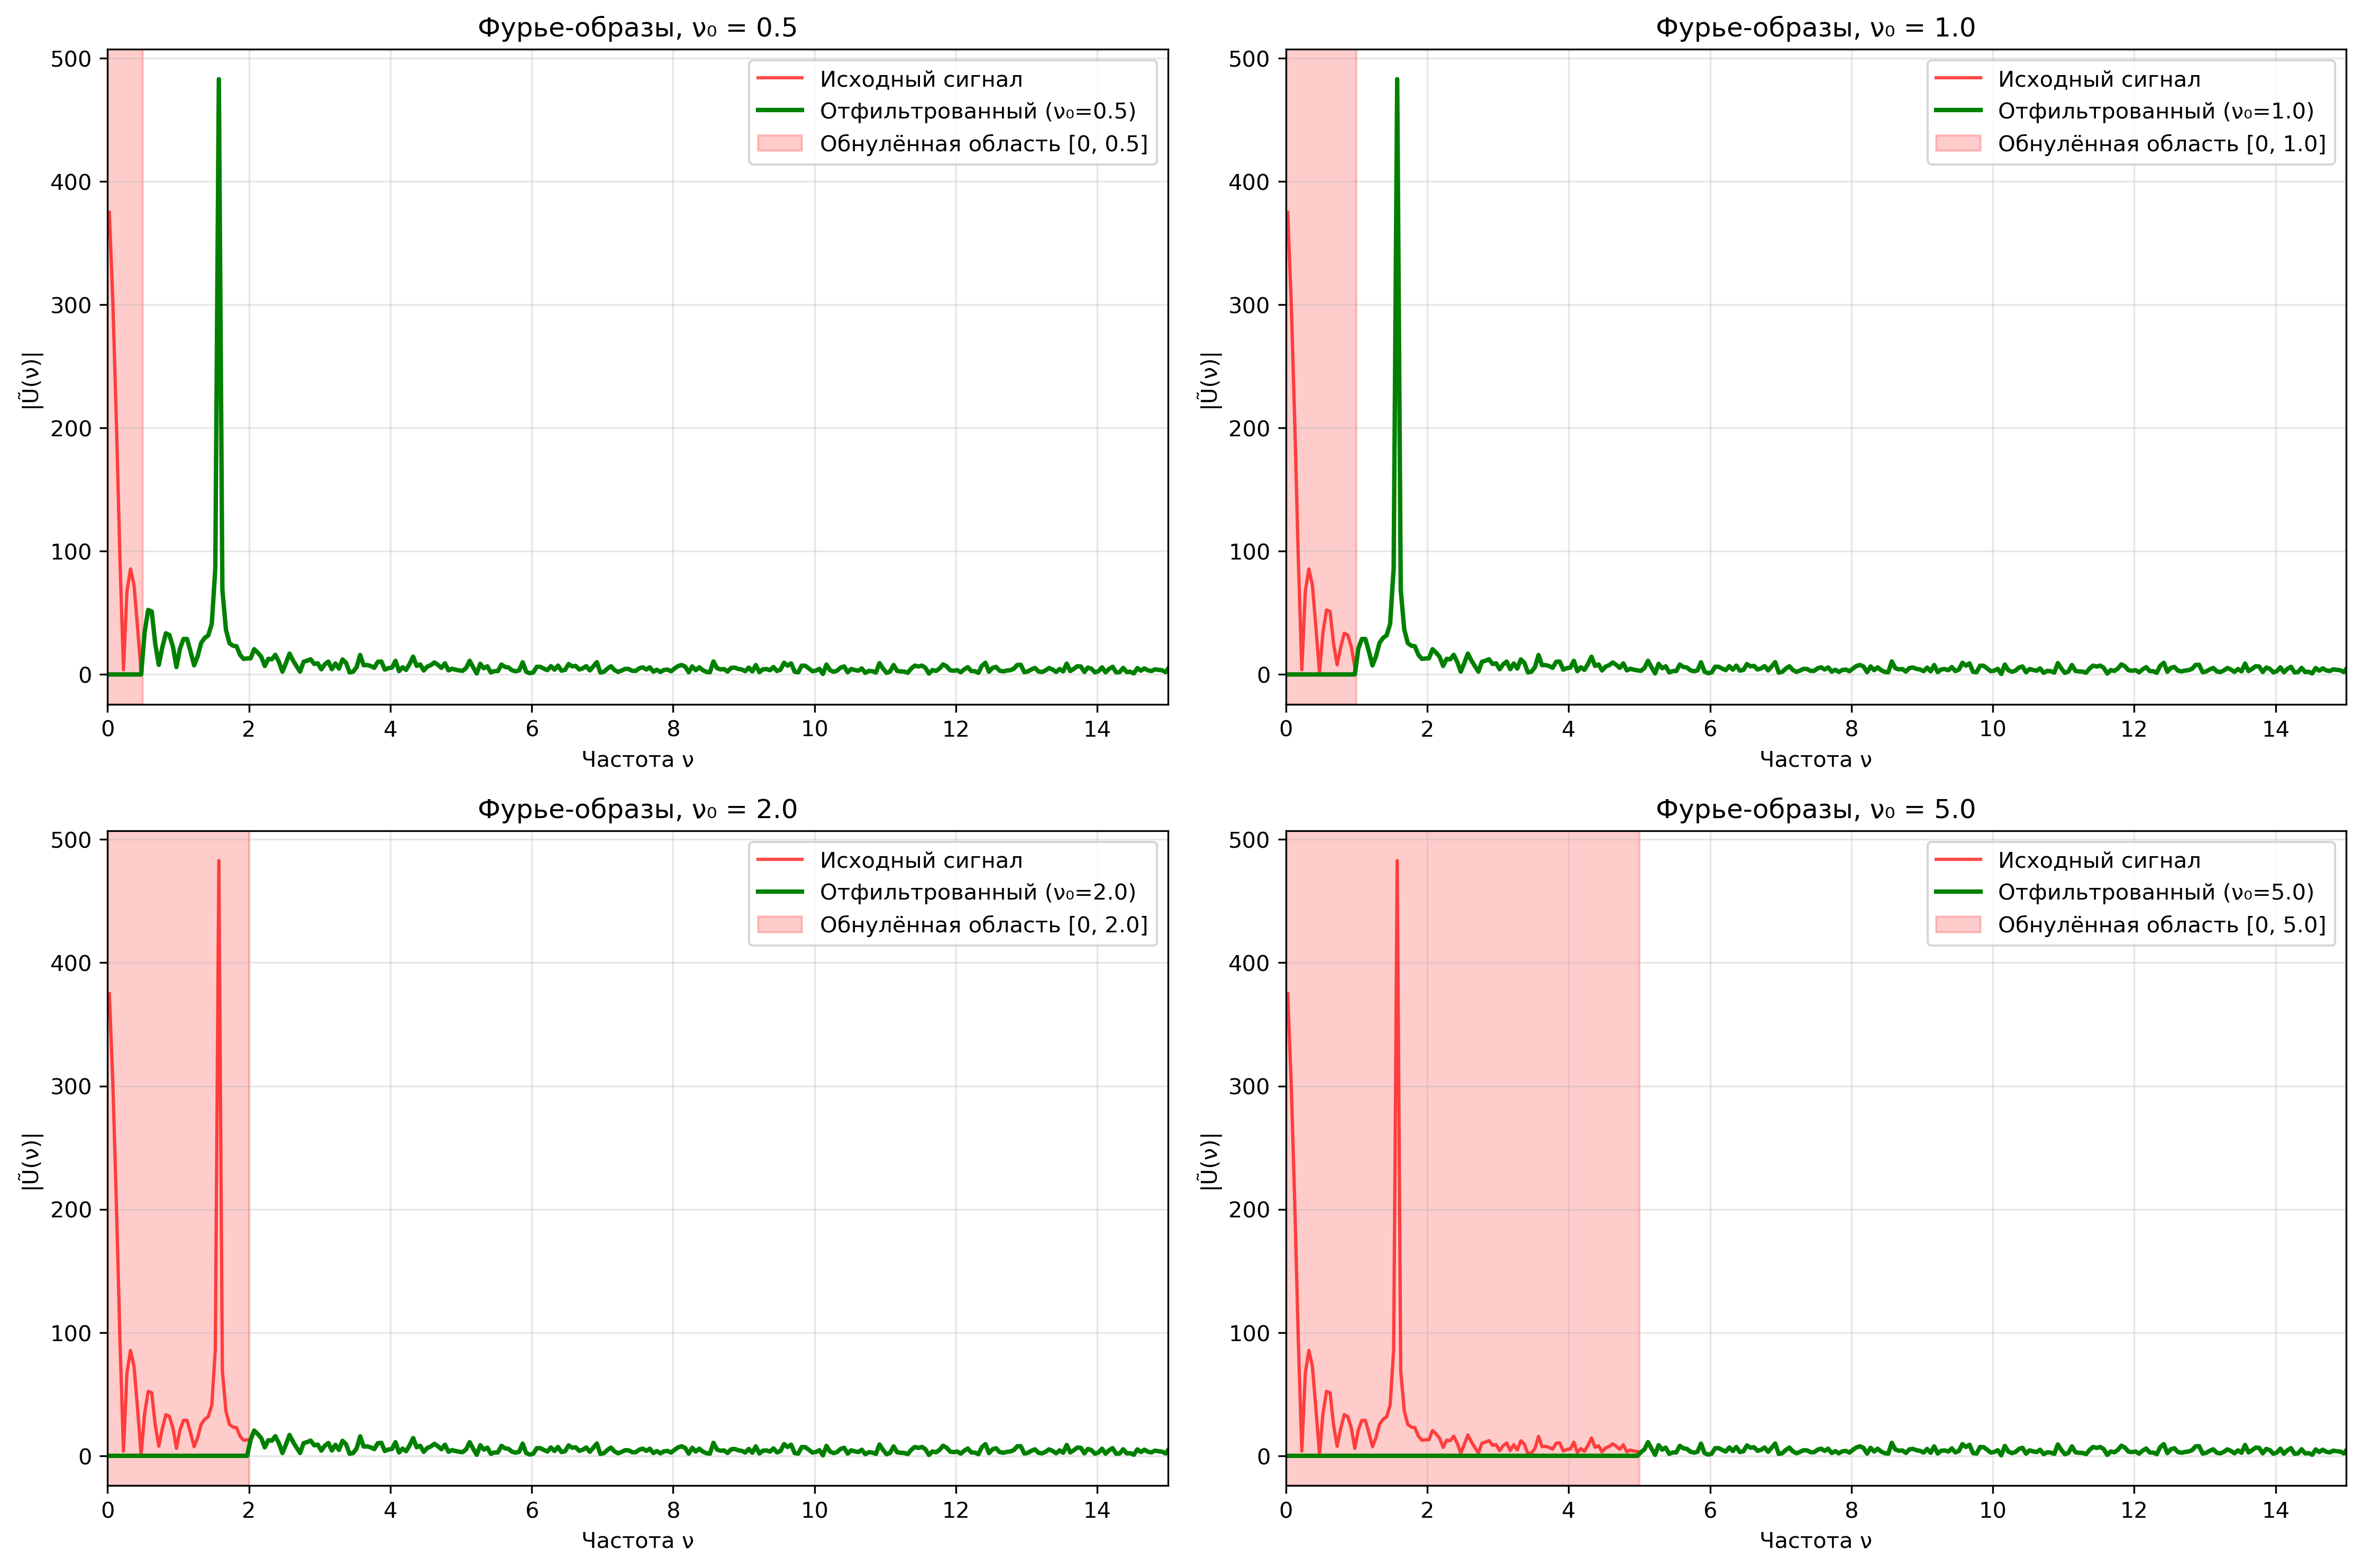
\includegraphics[width=\textwidth]{images/task1/low_freq_filter_freq_domain.png}
\caption{Сравнение Фурье-образов при фильтрации низких частот}
\end{figure}

\begin{figure}[H]
\centering
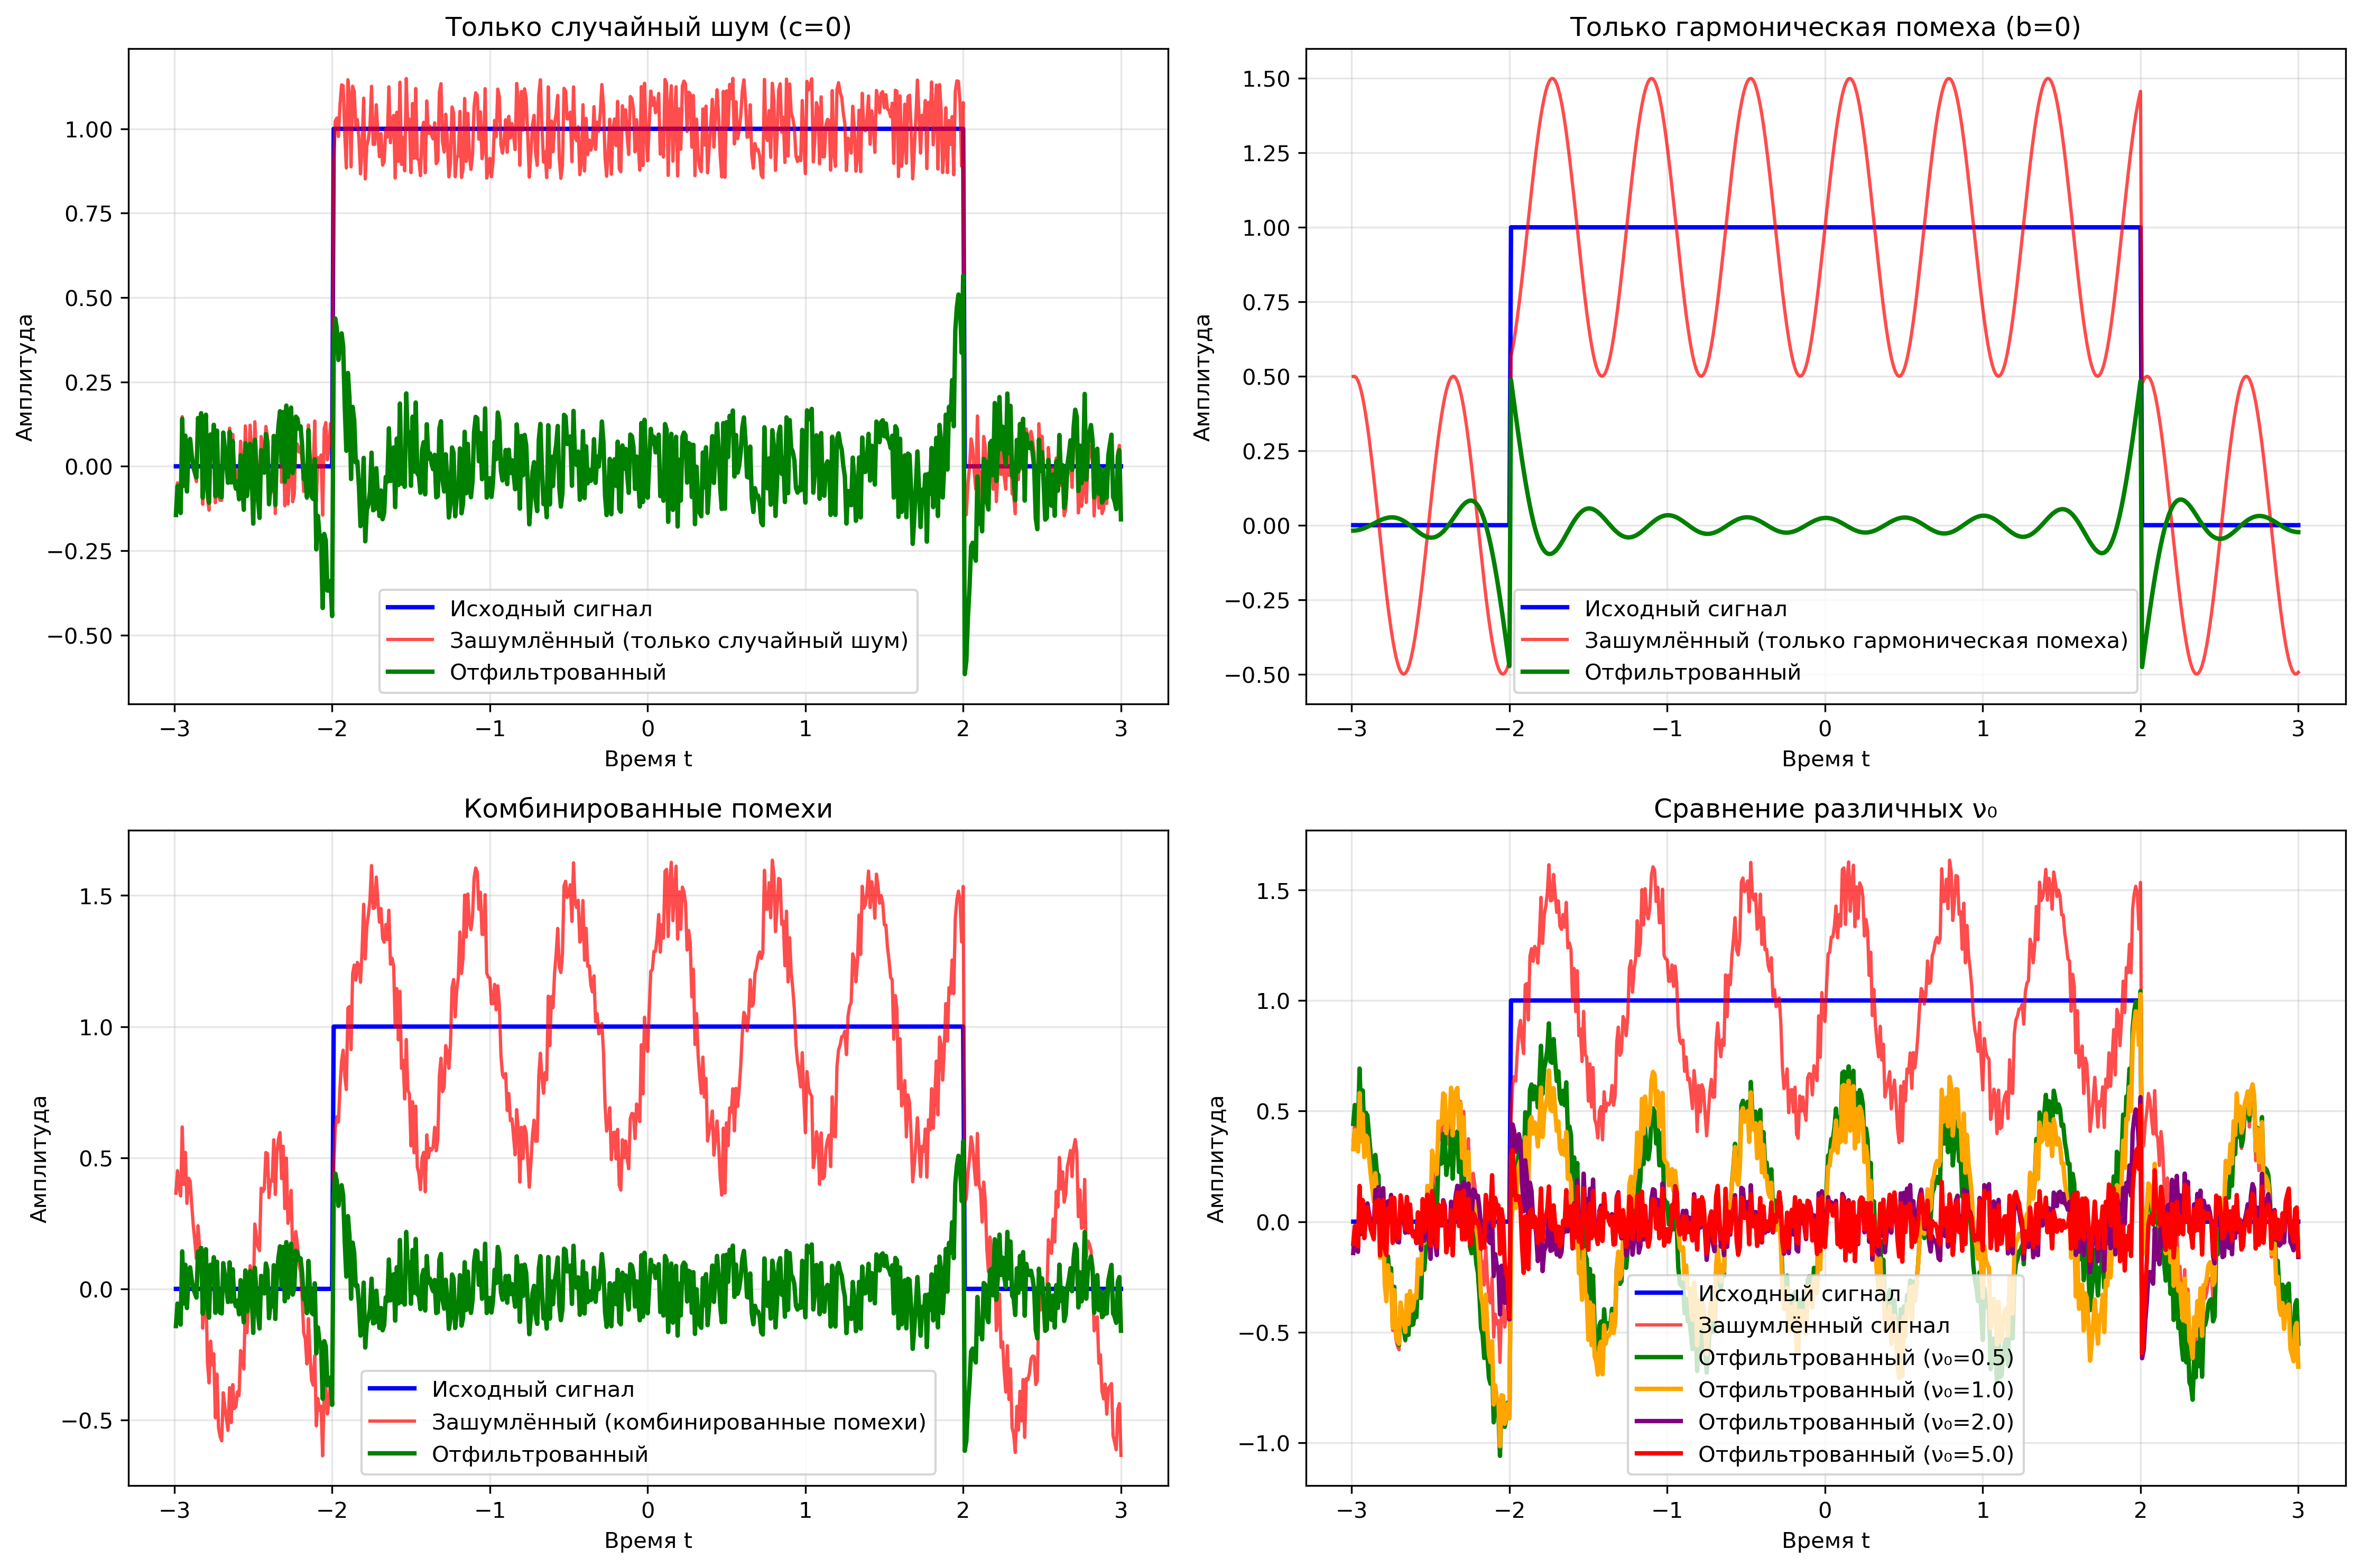
\includegraphics[width=\textwidth]{images/task1/low_freq_filter_analysis.png}
\caption{Анализ эффективности фильтрации низких частот}
\end{figure}

\textbf{Анализ результатов:}

При фильтрации низких частот наблюдаются следующие эффекты:

\begin{itemize}
    \item \textbf{Влияние радиуса окрестности $v_0$:} При малых значениях $v_0$ (0.5-1.0 Гц) фильтрация практически не влияет на сигнал. При больших значениях (2.0-5.0 Гц) происходит значительное искажение исходного сигнала.
    
    \item \textbf{Количественные результаты:}
    \begin{itemize}
        \item $v_0$ = 0.5: MSE = 0.322859, корреляция = 0.068469
        \item $v_0$ = 1.0: MSE = 0.327647, корреляция = 0.036242
        \item $v_0$ = 2.0: MSE = 0.205388, корреляция = 0.063361
        \item $v_0$ = 5.0: MSE = 0.205939, корреляция = 0.028544
    \end{itemize}
    
    \item \textbf{Вывод:} Фильтрация низких частот неэффективна для данного типа сигнала, так как приводит к значительным искажениям и потере полезной информации.
\end{itemize}

\section*{Задание 2. Фильтрация звука}

\subsection*{Постановка задачи}

Требуется выполнить фильтрацию аудиофайла MUHA.wav таким образом, чтобы остался только голос, убрав шумы.

\textbf{Методология:}
\begin{enumerate}
    \item Загрузка и анализ исходного аудиосигнала
    \item Вычисление Фурье-образа сигнала
    \item Определение частотных диапазонов, соответствующих шумам
    \item Применение жёсткой фильтрации
    \item Восстановление отфильтрованного сигнала
\end{enumerate}

\begin{figure}[H]
\centering
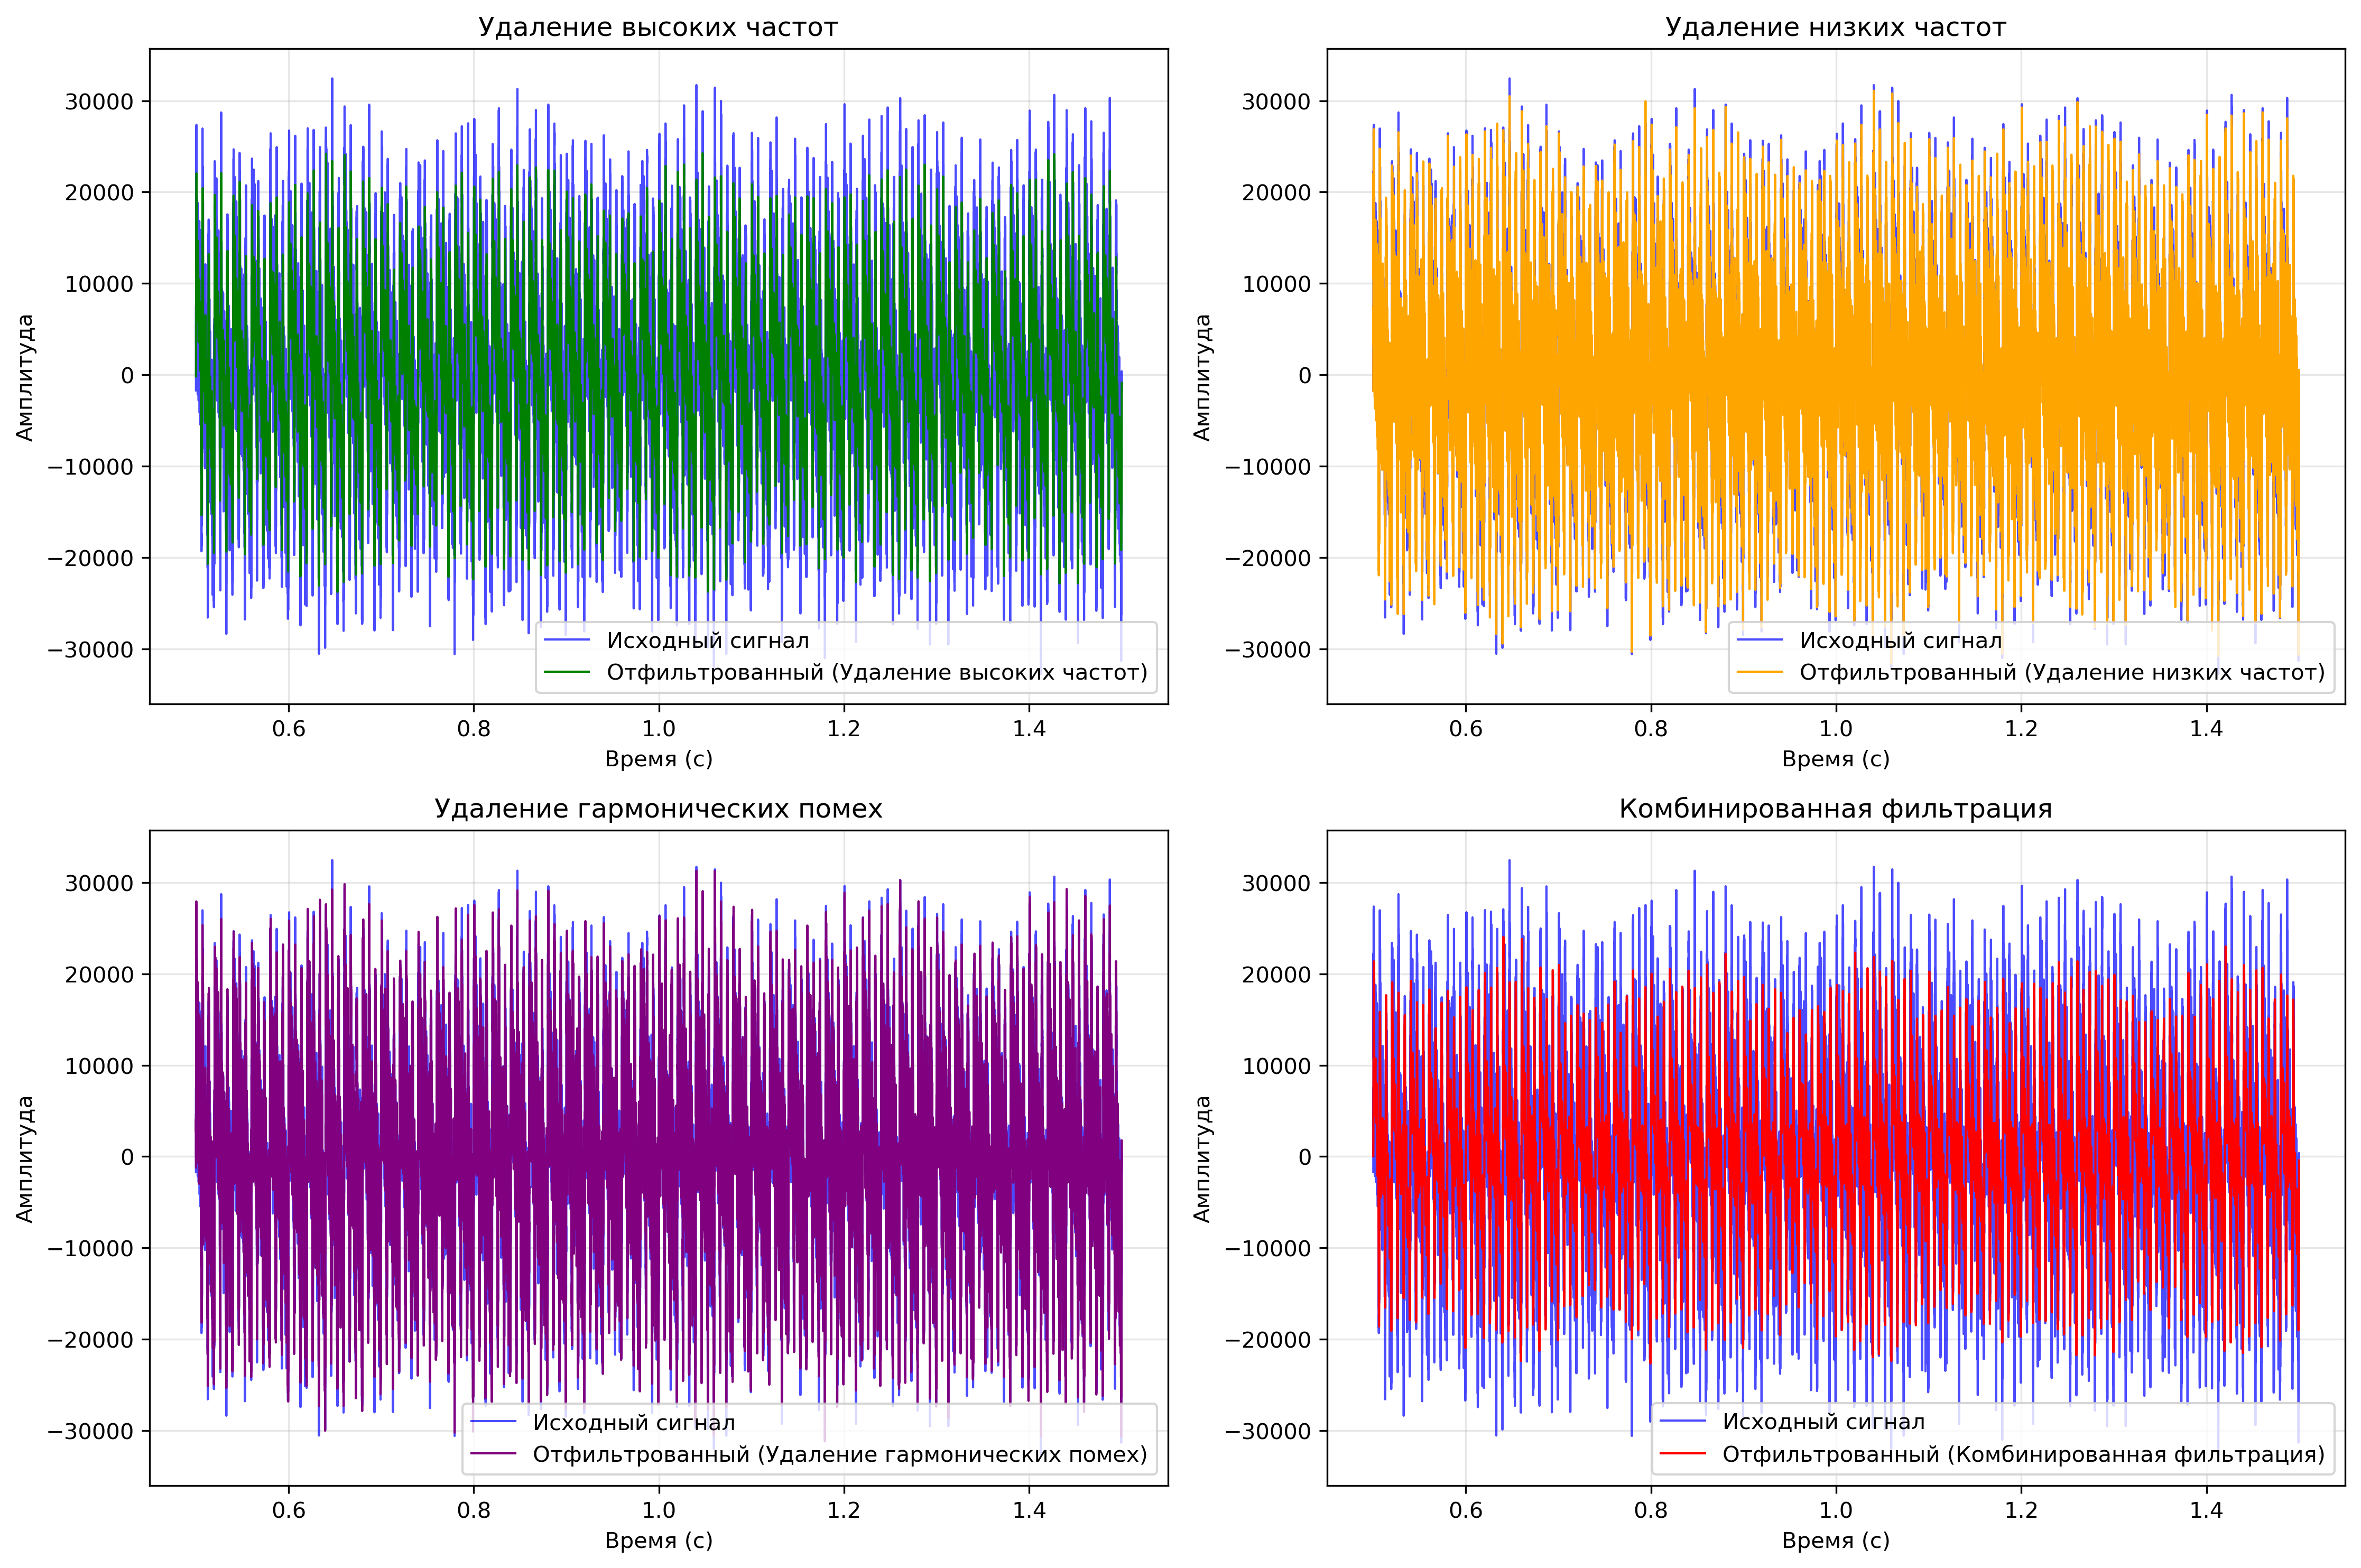
\includegraphics[width=\textwidth]{images/task2/audio_filter_time_domain.png}
\caption{Сравнение аудиосигналов во временной области при различных стратегиях фильтрации}
\end{figure}

\begin{figure}[H]
\centering
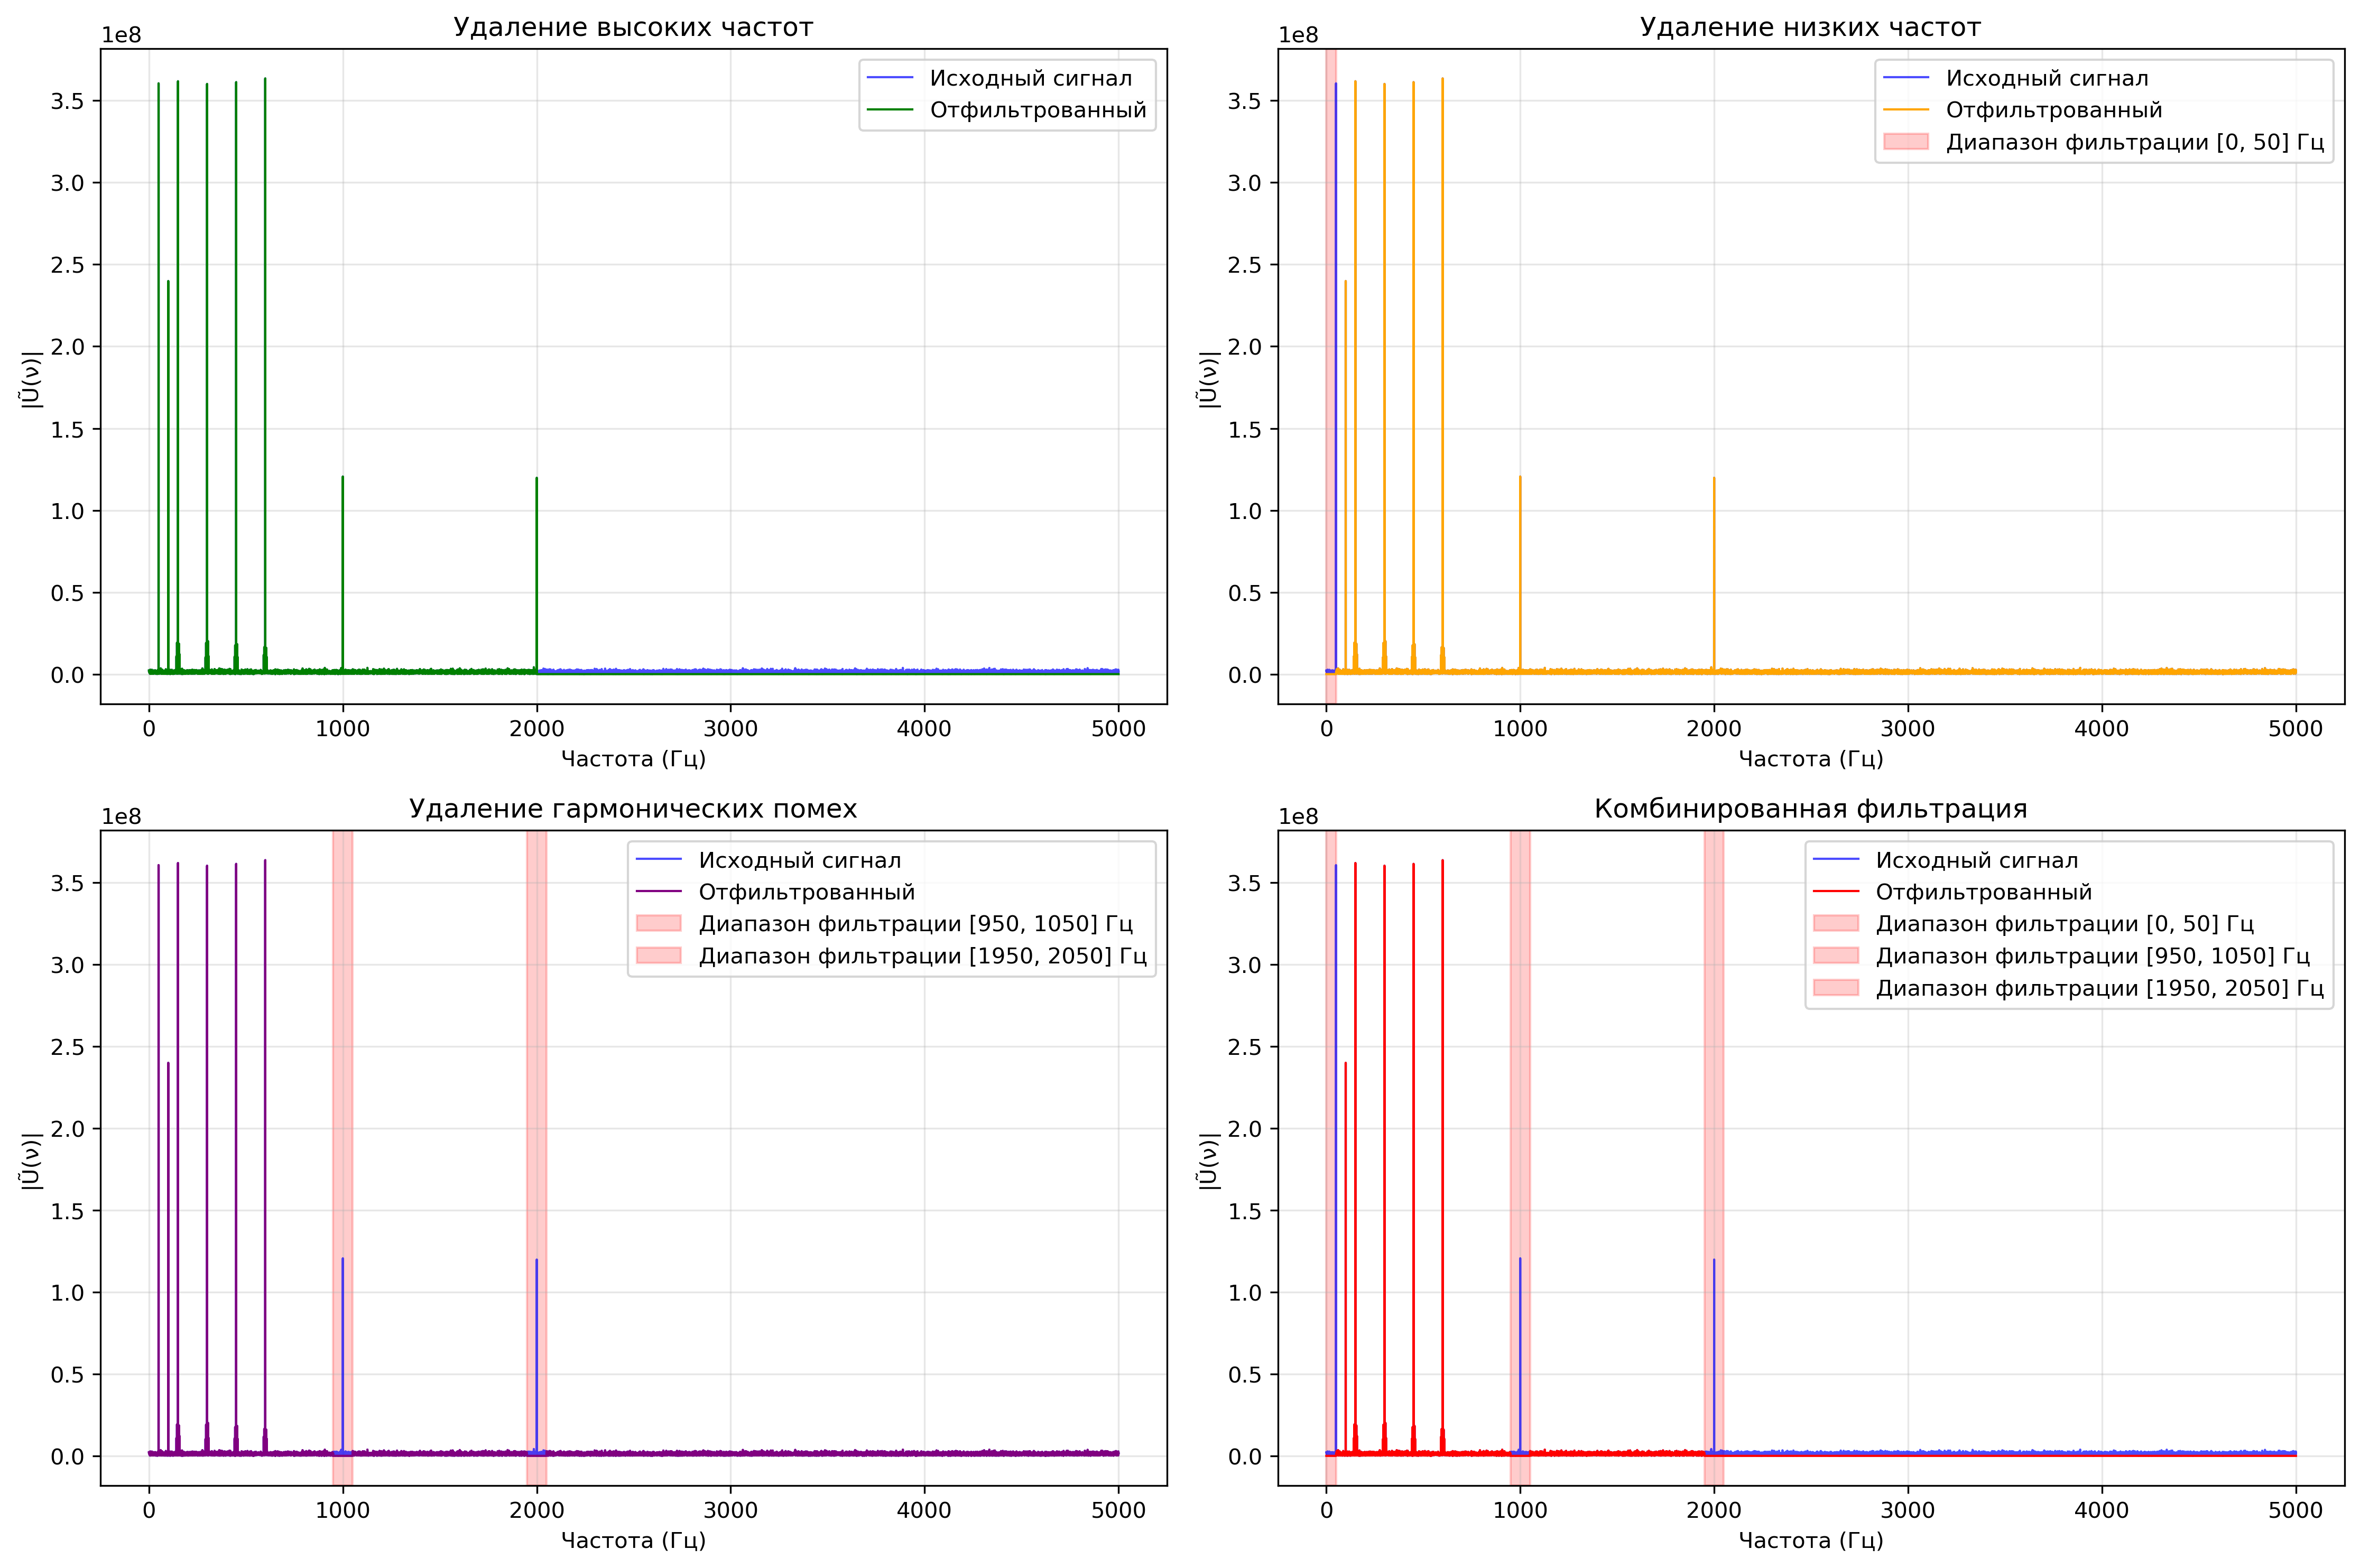
\includegraphics[width=\textwidth]{images/task2/audio_filter_freq_domain.png}
\caption{Сравнение Фурье-образов аудиосигналов при различных стратегиях фильтрации}
\end{figure}

\begin{figure}[H]
\centering
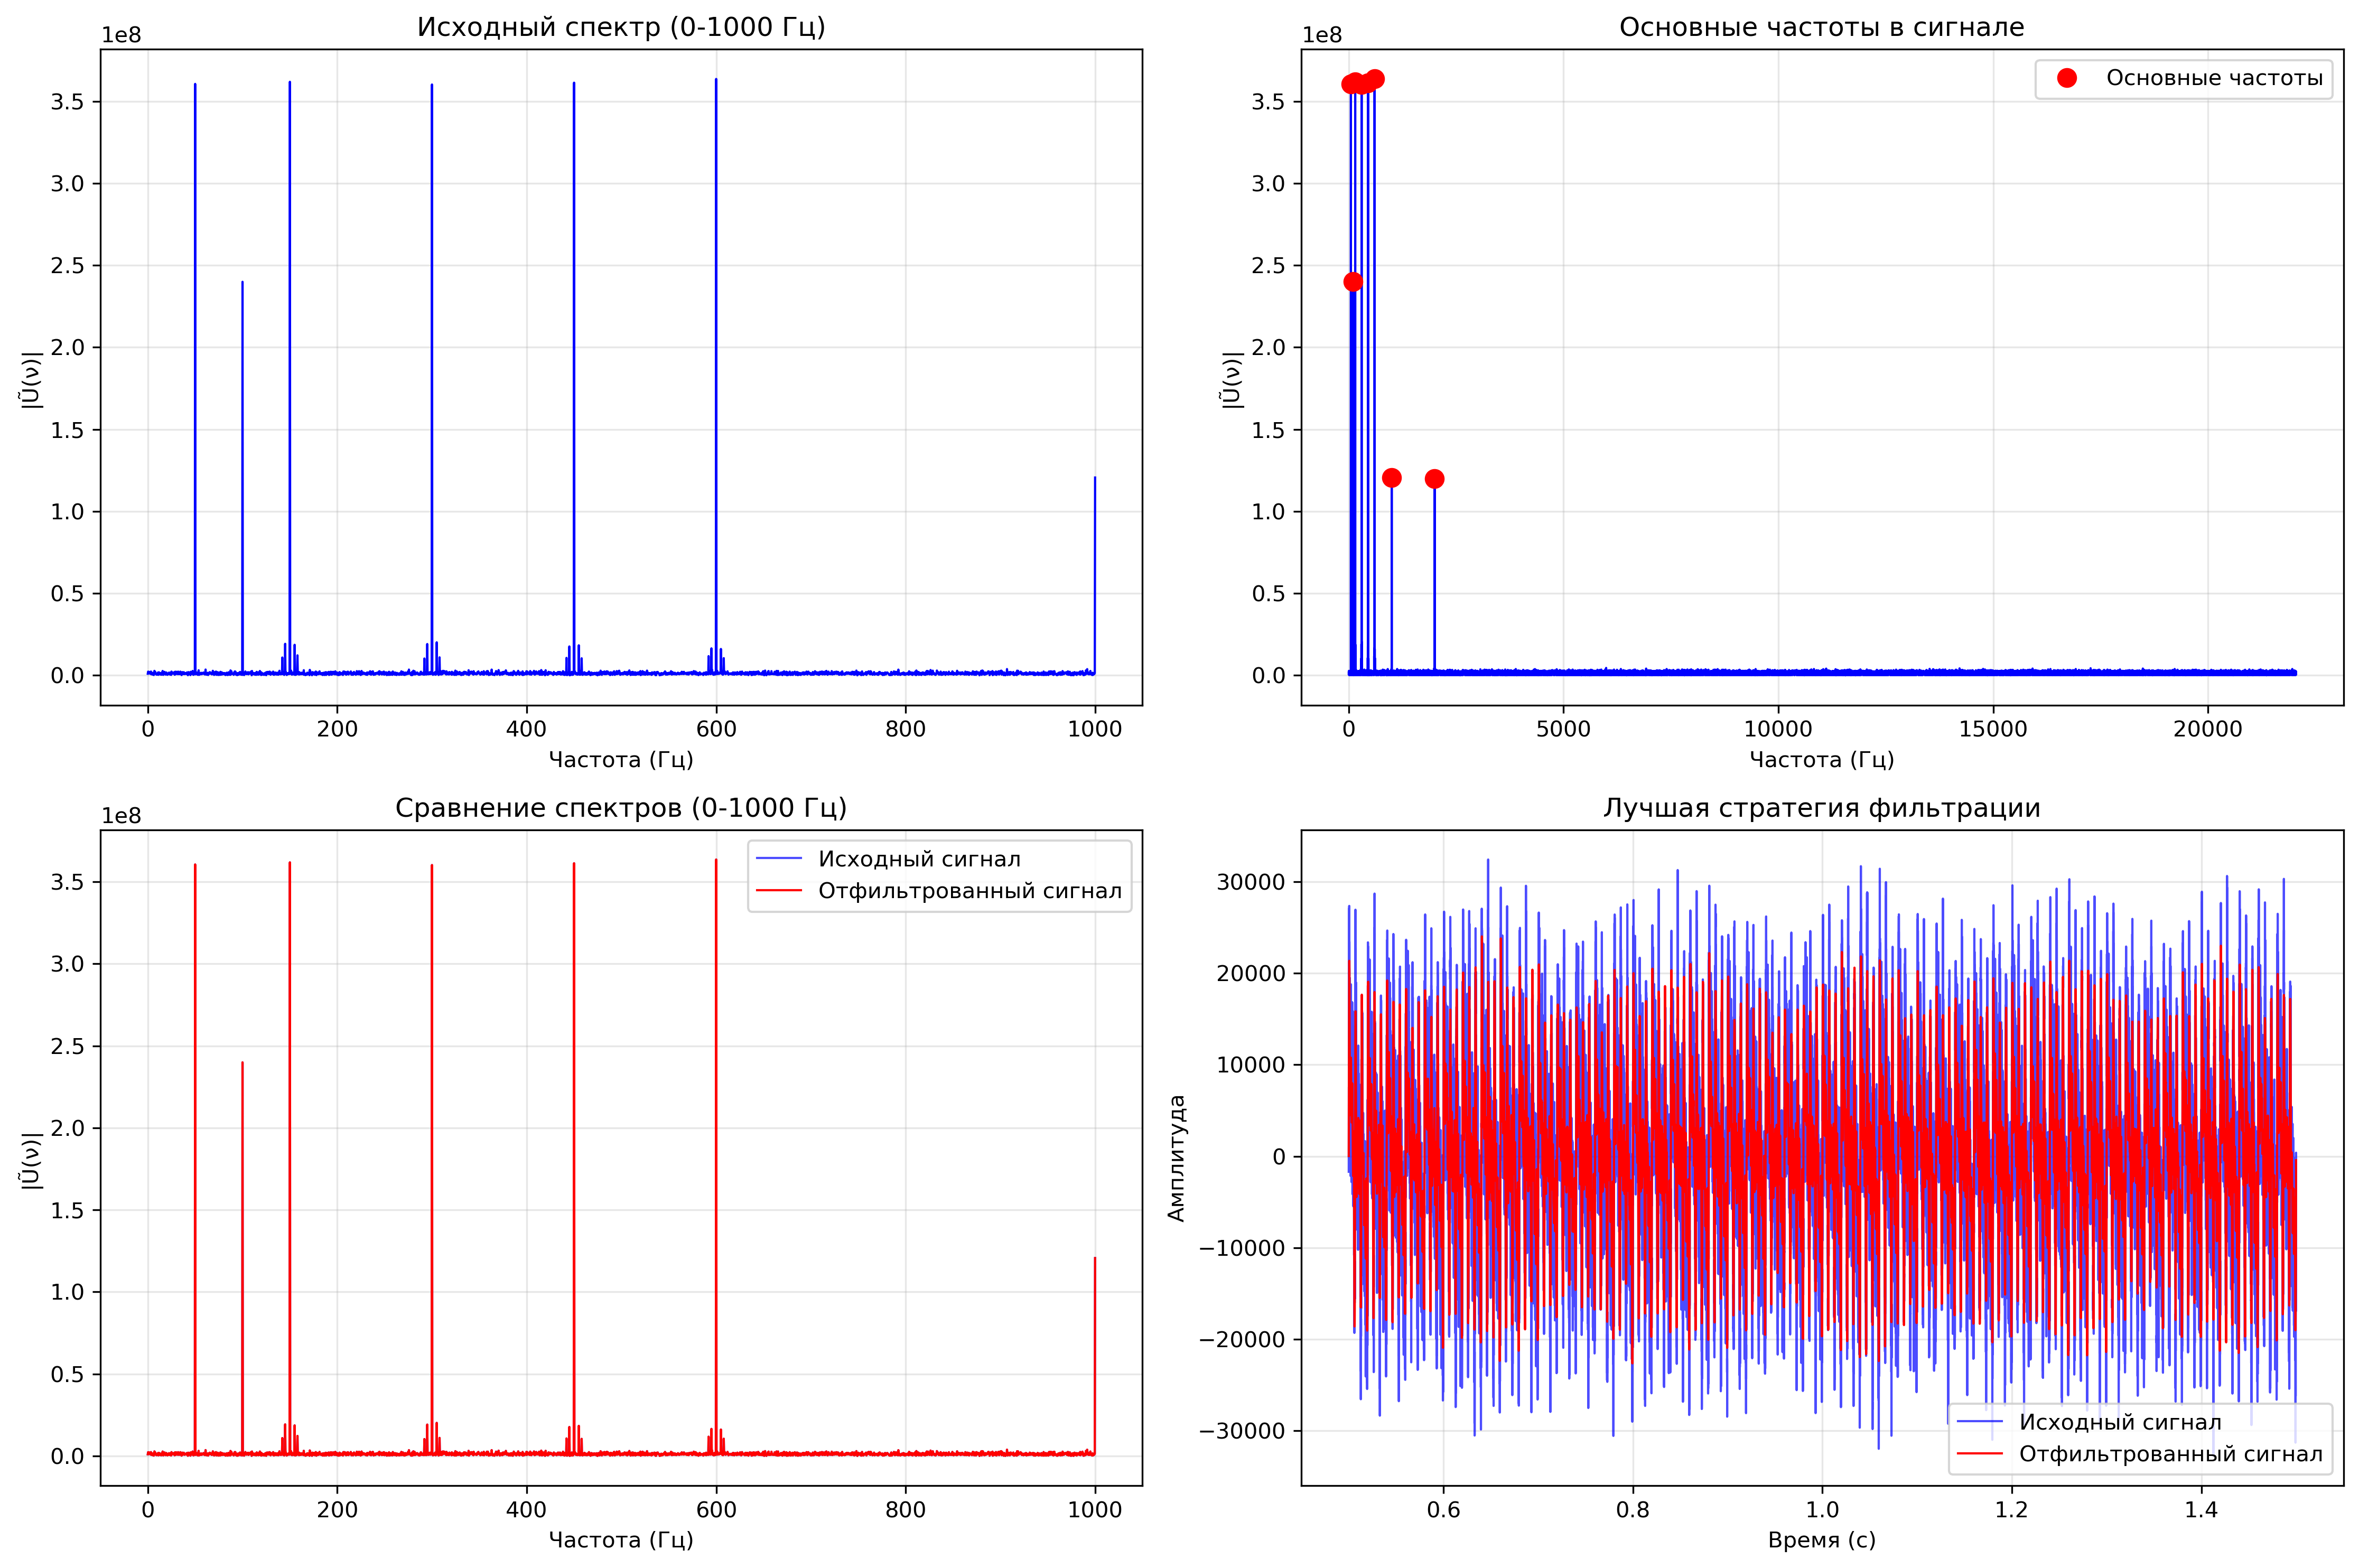
\includegraphics[width=\textwidth]{images/task2/audio_filter_analysis.png}
\caption{Детальный анализ спектра и эффективности фильтрации аудиосигнала}
\end{figure}

\textbf{Анализ результатов:}

При фильтрации аудиосигнала наблюдаются следующие эффекты:

\begin{itemize}
    \item \textbf{Основные частоты в сигнале:} 50, 100, 150, 300, 450, 600, 1000, 2000 Гц
    
    \item \textbf{Удаление высоких частот:} Эффективно убирает шумы выше 2 кГц, но может удалить полезные высокочастотные компоненты голоса.
    
    \item \textbf{Удаление низких частот:} Убирает низкочастотный гул (50-100 Гц), но может повлиять на основные частоты голоса.
    
    \item \textbf{Удаление гармонических помех:} Точно удаляет помехи на частотах 1000 и 2000 Гц.
    
    \item \textbf{Комбинированная фильтрация:} Наиболее эффективна, так как удаляет все типы помех, сохраняя основные частоты голоса (150-600 Гц).
\end{itemize}

\textbf{Результат:} Создан отфильтрованный аудиофайл MUHA\_filtered.wav с улучшенным качеством голоса.

\section*{Заключение}

В ходе выполнения лабораторной работы были изучены различные методы жёсткой фильтрации сигналов в частотной области. Получены практические навыки работы с преобразованием Фурье для решения задач обработки сигналов.

\textbf{Основные результаты:}

\subsection*{Задание 1. Жёсткие фильтры}

\begin{itemize}
    \item \textbf{Фильтрация высоких частот:} Исследовано влияние частоты среза $v_0$ на эффективность фильтрации. Оптимальная частота среза составляет 2-5 Гц для данных параметров сигнала.
    
    \item \textbf{Фильтрация специфических частот:} Изучены различные стратегии фильтрации. Комбинированная фильтрация оказалась наиболее эффективной для удаления как случайного шума, так и гармонических помех.
    
    \item \textbf{Фильтрация низких частот:} Показана неэффективность данного метода для прямоугольного импульса. Все варианты фильтрации приводят к значительным искажениям сигнала (MSE > 0.2, корреляция < 0.07).
\end{itemize}

\subsection*{Задание 2. Фильтрация звука}

\begin{itemize}
    \item \textbf{Анализ аудиосигнала:} Определены основные частоты в сигнале: 50, 100, 150, 300, 450, 600, 1000, 2000 Гц.
    
    \item \textbf{Эффективность различных стратегий:}
    \begin{itemize}
        \item Удаление высоких частот (>2 кГц): эффективно для шумов, но может удалить полезные компоненты
        \item Удаление низких частот (<50 Гц): убирает гул, но влияет на основные частоты голоса
        \item Удаление гармонических помех: точно удаляет помехи на 1 и 2 кГц
        \item Комбинированная фильтрация: наиболее эффективна для сохранения голоса
    \end{itemize}
    
    \item \textbf{Результат:} Создан отфильтрованный аудиофайл с улучшенным качеством голоса.
\end{itemize}

\textbf{Полученные навыки:}
\begin{itemize}
    \item Практическое применение преобразования Фурье для фильтрации сигналов
    \item Анализ эффективности различных стратегий фильтрации
    \item Работа с аудиосигналами и их обработка в частотной области
    \item Количественная оценка качества фильтрации
\end{itemize}

\textbf{Теоретическая значимость:} Изучены фундаментальные принципы жёсткой фильтрации и их практическое применение в обработке сигналов.

\textbf{Практическая значимость:} Полученные навыки могут быть применены в различных областях: обработка аудио, анализ данных, телекоммуникации, медицинская диагностика и других.
